
\section{Introducción y conceptos previos}
Una ecuación diferencial es una ecuación matemática que relaciona una función con sus derivadas. En las matemáticas aplicadas, las funciones usualmente representan cantidades físicas, las derivadas representan sus razones de cambio y la ecuación define la relación entre ellas. Como estas relaciones son muy comunes, las ecuaciones diferenciales juegan un rol primordial en diversas disciplinas, incluyendo la ingeniería, la física, la química, la economía y la biología.

En las matemáticas puras, las ecuaciones diferenciales se estudian desde perspectivas diferentes, la mayoría concernientes al conjunto de las soluciones de las funciones que satisfacen la ecuación. Solo las ecuaciones diferenciales más simples se pueden resolver mediante fórmulas explícitas; sin embargo, se pueden determinar algunas propiedades de las soluciones de una cierta ecuación diferencial sin hallar su forma exacta.

En esta primera parte, se expondrá un marco teórico necesario en el que encuadrar las soluciones de ecuaciones diferenciales, los campos vectoriales, los espacios tangentes y cotangentes (y las aplicaciones tangentes y cotangentes asociadas) y las 1-formas enmarcadas en los espacios duales.
\begin{eje}
Dada la ecuación diferencial
$$y'(x)=f(x)$$
una solución viene dada por la \textbf{cuadratura}:
$$y(x)=\int f(x) \: dx + C$$
Es decir, si $f$ es continua (más general, integrable Riemann), la ecuación tiene al menos una solución, y el resto se obtienen sumando constantes.
\end{eje}
\begin{eje}
Consideremos la ecuación $y'=y$ (que modela la desintegración radiactiva, por ejemplo), luego algunas soluciones son 
$$y=e^x \qquad y=0 \qquad y=e^{x+c}$$
luego podemos generalizar la solución como $y=c \: e^x \: / \: c \in \mathbb{R}$. Veamos si existen más soluciones. Sean $y_i'=y_i$ con $i=\{1,2\}$ dos soluciones:
$$\left( \dfrac{y_1}{y_2} \right)'=\dfrac{y_1'y_2-y_1y_2'}{y_2^2}=\dfrac{y_1y_2-y_1y_2}{y_2^2}=0 \iff y_1=c\: y_2$$
\end{eje}
Estudiaremos ecuaciones de la forma $y'=f(x,y)$, llamadas ecuaciones diferenciales ordinarias de 1$^{\text{er}}$ orden.

Sea $y'=f(x,y)$ una ecuación diferencial,
\begin{defi}
Llamamos \textbf{solución} a una función derivable $\phi(x)$ tal que sustituida por $y$ en la ecuación de lugar a una identidad:
$$\phi'(x)=f(x,\phi(x))$$
Decimos entonces que ``$y=\phi(x)$ es un solución''.
\end{defi}
\section{Campos de vectores}
Sea $U \subset \mathbb{R}^n$
\begin{defi}
    Un \textbf{campo de vectores} es un aplicación:
    $$\begin{array}{rcl}
         U & \overset{v}{\longrightarrow} & \mathbb{R}^n \\
         p & \longmapsto & v_p 
    \end{array}$$
asignando así a cada punto del espacio un vector.    
\end{defi}
\begin{ejes} \: 
\begin{enumerate} 
    \item $v_{(x,y)}:=(-y,x)$ 
    \item $v_{(x,y)}:=(1,y)$
\end{enumerate}
\end{ejes}
\begin{nota}
Los campos vectoriales modelan fenómenos físicos, como campos magnéticos, eléctricos, de fluidos, etc.
\end{nota}
\begin{obs}
Dada una ecuación diferencial, $y'=f(x,y)$, asignando a cada $(x,y)\longmapsto (1,f(x,y))$ obtenemos una correspondencia biunívoca con un campo de vectores.
\end{obs}
\subsection{Vectores, derivadas direccionales y vectores tangentes}
\begin{defi}
    Dado $p \in U \subseteq \mathbb{R}^n$ y $v$ un vector de $\mathbb{R}^n$, definimos la \textbf{derivada direccional} $$D_{p,v}F:=\left.\dfrac{dF(p+tv)}{dt}\right|_{t=0}$$
    De forma que como aplica a funciones $F$, definimos la derivada direccional entre $\mc{C}^{\infty}(U)\longrightarrow \mathbb{R}$.
\end{defi}
\begin{ejes}
    \begin{enumerate}
        \item Dado el campo vectorial $v_{(x,y)}=(1,0)$, $D_{p,v}F=\left(\pd{F}{x}\right)_p$, luego
        $$v=(1,0) \longmapsto D_{p,v}=\left( \pd{}{x}\right)_p$$
        \item Si $v=(1,y)$,
        $$D_{p,v}F=d_pF \: \: \: (1,y)=\left( \left(\pd{F}{x}\right)_p \quad \left(\pd{F}{y}\right)_p\right) {1 \choose y}=\left(\pd{F}{x}\right)_p+y\left(\pd{F}{y}\right)_p$$
    \end{enumerate}
\end{ejes}
\begin{propi}
Dado que $D_{p,v}:\mc{C}^{\infty}(U) \longrightarrow \mathbb{R}$ cumple las propiedades:
\begin{enumerate}
    \item $D_{p,v}(\alpha F + \beta G)=\alpha D_{p,v}F + \beta D_{p,v} G$
    \item $D_{p,v}(F\cdot G)=F(p)D_{p,v}G+G(p)D_{p,v}F$
\end{enumerate}
llamamos a $D_{p,v}$ una $\mathbb{R}$-\textbf{derivación}, teniéndose que
$$D_p=D_px_1\left(\pd{}{x_1}\right)_p + D_px_2\left(\pd{}{x_2}\right)_p + \cdots + D_px_n\left(\pd{}{x_n}\right)_p $$
\end{propi}
\begin{prop}
La derivada direccional esinvariante respecto a los cambios de coordenadas, es decir, se verifica que $$D_p=\sum_i D_px_i \left( \pd{}{x_i}\right)_p=D_p\psi_1\left(\pd{}{\psi_1}\right)_p + D_p\psi_2\left(\pd{}{\psi_2}\right)_p + \cdots + D_p\psi_n\left(\pd{}{\psi_n}\right)_p $$
\end{prop}
\begin{dem}
Por las fórmulas del cambio de variable,
$$\pd{}{x_i}=\sum_{j} \pd{\psi_j}{x_i} \pd{}{\psi_j}$$
luego sustituyendo en $D_p$ expresado en cartesianas, 
$$\sum_i D_px_i \left(\pd{}{x_i} \right)_p=\sum_i D_px_i \left(\sum_{j} \pd{\psi_j}{x_i} \pd{}{\psi_j}\right)_p=\sum_j \underbrace{\left( \sum_i D_px_i \left( \pd{\psi_j}{x_i}\right)_p\right)}_{D_p\psi_j} \left( \pd{}{\psi_j}\right)_p=$$
\end{dem}
\begin{eje}
    Se pide expresar $D_p=\left( -y \pd{}{x} + x \pd{}{y}\right)_p$ en polares. 
\end{eje}
\begin{sol}
$D_p=D_pr \pd{}{r} + D_p \theta \pd{}{\theta}$
$$D_pr=D_p \sqrt{x^2+y^2}=\dfrac{1}{2\sqrt{x^2+y^2}}(2x D_px+2yD_py)=\dfrac{1}{2\sqrt{x^2+y^2}}(2x(-y)+2yx)=0$$
$$D_p \theta = D_p(\arctan(\nicefrac{y}{x}))=\dfrac{1}{1+(\nicefrac{y}{x})^2}D_p(\nicefrac{y}{x})=\dfrac{1}{1+(\nicefrac{y}{x})^2} \dfrac{\cancelto{x}{D_y} x - y \cancelto{-y}{D_px}}{x^2}=1$$
\end{sol}
\section{Espacio tangente y cotangente}
\begin{defi}
    Considerando el conjunto de los operadores $D_{p,v}: \mc{C}^{\infty}(U) \longrightarrow \mathbb{R}$, 
    $$\{D_{p,v} \: | \: v \in \mathbb{R}^n\}=: T_pU$$
    que llamaremos \textbf{espacio tangente} a $U$ en $p$.
    De esta forma, existe un isomorfismo
    $$\begin{array}{rcl}
         \mathbb{R}^n & \overset{\sim}{\longrightarrow} & T_pU  \\
         v & \longmapsto & D_{p,v}  
    \end{array}$$
\end{defi}
Podemos generalizar este espacio tangente a campos vectoriales, como sigue.
\begin{defi}
    Dado el campo $v: U \longrightarrow \mathbb{R}^n$, quedando definido el campo de vectores tangente: $p \longmapsto D_{p, v(p)} \in T_pU$
\end{defi}
\begin{eje}
    Sea $U=\mathbb{R}_{x,y}^2$ y $$p=(x,y) \longmapsto v(p)=(e^{xy}, x-\cos \: y)_p \longmapsto \left(e^{xy} \pd{}{x} + (x-\cos \: y) \pd{}{y}\right)_p $$
\end{eje}
\begin{obs}
    En general, los campos de vectores tangentes se espresan como 
    $$D=\sum_{i} \alpha_i(x_1, \ldots, x_n) \pd{}{x_i}$$
\end{obs}
\begin{nota}
    De esta forma, podemos definir $D_pF$ como composición de funciones:
    $$\begin{array}{rrrll}
         \mc{C}^{\infty}(U) & \overset{D}{\longrightarrow} & \mc{C}^{\infty}(U)    \\
         F & \longmapsto & DF:U & \longrightarrow & \mathbb{R} \\
         & & p & \longmapsto & D_pF
    \end{array}$$
\end{nota}
\begin{defi}
    Dado $T_pU$, podemos definir el espacio vectorial de $T_pU$, $T_p^{*}U$ que llamamos \textbf{espacio cotangente} y donde cada $\omega_p \in T_p^*U$ se denomina \textbf{covector}.

    Si $F\in \mc{C}^{\infty}(U)$, tenemos el siguiente covector:
    $$\begin{array}{rcl}
        T_pU & \overset{d_pF}{\longrightarrow} & \mathbb{R}  \\
        D_p & \longrightarrow & D_pF 
    \end{array}$$
    Es decir, $d_pF(D_p):=D_pF$ y donde $d_pF \in T^*_pU$ es lineal. 
\end{defi}
\begin{nota}
    ¿Qué coño tiene todo esto que ver con la derivada de $F$?
\end{nota}
\begin{prop}
    $$\begin{tikzcd}
    & D_{p,v} \ar[mapsto]{rr} &  & d_pF(D_{p,v})& \arrow[equal]{l}D_{p,v}F \\
    D_{p,v} & T_pU \ar{rr}{d_pF} & & \mathbb{R} \\
    & & & d_pF(v) & D_{p,v} F \arrow[l, equal] \arrow[uu, equal] \\
    v \arrow[uu, mapsto]  & \mathbb{R}^n \ar{uu}{\sim} \ar[rruu, dashrightarrow] & &  & \\
    & v \arrow[mapsto]{rruu}{d_pF}  &  
    \end{tikzcd}$$
\end{prop}
En particular si $x_1, \ldots, x_n$ son las funciones coordenadas, cosntruimos $d_px_1, \ldots, d_px_n$ una base de $T_p^*U$. Consideremos 
$$\begin{array}{rcl}
     T_pU& \overset{d_pF}{\longrightarrow} & \mathbb{R}  \\
     \left(\pd{}{x_i} \right)_p & \longmapsto & \left(\pd{F}{x_i}\right)_p \quad \forall i \in \{1, \ldots, n\}
\end{array}$$
de forma que $d_px_i: T_pU \longrightarrow \mathbb{R}$ es $$d_px_i\left(\pd{}{x_j}\right)=\delta_{ij}$$
por tanto, $\{d_px_i\}_{i=\{1,\ldots,n\}}$ es la base dual de $\{\left(\pd{}{x_i}\right)\}_{i=\{1,\ldots,n\}}$. Además, dado que los cambios de coordenadasson ``buenos'', tenemos que $\{d_p\psi_i\}_{i=\{1,\ldots,n\}}$ es la base dual de $\{\left(\pd{}{\psi_i}\right)\}_{i=\{1,\ldots,n\}}$
\begin{defi}
    Así pues, igual que con vectores, podemos definir \textbf{campos de covectores o 1-formas diferenciales} en $U$, es la aplicación
    $$U \ni p \overset{\omega}{\longmapsto} \omega_p \in T_p^*U$$
    de forma que 
    $$\omega_p=A_1(p) \: d_px_1 + \cdots + A_n(p) \: d_px_n$$
    teníendose así $n$ funciones $A_i$, y pondremos
    $$\omega=A_1 \: dx_1 + \cdots + A_n \: dx_n$$
\end{defi}
\begin{eje}\:
    \begin{enumerate}
        \item Si $\omega=dx_1$, $p \overset{dx_1}{\longmapsto} d_px_1 \in T^*_pU$.
        \item Si $\omega =x_2 dx_1$, 
        $$\begin{array}{rcl}
             p & \longmapsto & x_2(p) \: d_px_1  \\
             (5,34) & \longmapsto & 34 \: d_{(5,34)}x_1
        \end{array}$$
        \item Sea $F \in \mc{C}^{\infty}(U)$, $p \overset{dF}{\longmapsto} d_pF \in T^*_pU$ donde $dF=\sum \frac{\partial F}{\partial x_i}\: dx_i$
    \end{enumerate}
\end{eje}
\begin{defi}
Un campo de vectores tangente $D=\sum \alpha_i(x_1, \ldots , x_n) \pd{}{x_i}$ se dice \textbf{de clase} $\mc{C}^{\infty}$ si $\alpha_1, \ldots, \alpha_n$ son funciones $\mc{C}^{\infty}$. Idem. para $\omega=A_1 \: dx_1 + \cdots + A_n \: dx_n$. 
\end{defi}
\section{Aplicaciones tangente y cotangente}
\begin{defi} Consideremos la aplicación de clase $\mc{C}^{\infty}(U)$
$$\begin{array}{rrcl}
     \gamma : & \mathbb{R}^n_{x_1, \ldots, x_n} \supseteq U & \longrightarrow & V \subseteq \mathbb{R}^m_{y_1, \ldots, y_m}  \\
     & (x_1, \ldots, x_n)=x & \longmapsto & \gamma(x)=(\gamma_1(x), \ldots, \gamma_m(x)) 
\end{array}$$
Observamos que en general
$$\begin{tikzcd}
    U \arrow[swap,dashed]{ddr}{\gamma^*G:=G\circ \gamma} \arrow{rr}{\gamma} & & V \arrow{ddl}{G} \\
    & & &\\
    & \mathbb{R} & 
\end{tikzcd}$$
y si $G$ es de clase $\mc{C}^{\infty}(V)$, se induce la aplicación
$$\begin{array}{rcl}
     \mc{C}^{\infty}(U) & \overset{\: \: \: \: \: \gamma^*}{\longleftarrow} & \mc{C}^{\infty}(V)   \\
     \gamma^* G & \longleftarrow & G 
\end{array}$$
Considerando $G=y_i$, $\gamma^*y_i=y_i \circ \gamma=\gamma_i$, la $i$-ésima coordenada de $\gamma$.

Esta aplicación $\gamma^*$ es la que llamaremos \textbf{aplicación tangente}.
\end{defi}

\begin{defi}
Considerando ahora $D_p \in T_pU$ tal que $D_p: \mc{C}^{\infty}(U) \longrightarrow \mathbb{R}$ definimos pues 
$$\begin{array}{rrclrll}
    \gamma_{*,p} : & T_pU & \longrightarrow & T_{\gamma(p)}V  \\
     & D_p & \longmapsto & \gamma_{*,p}(D_p):&  \mc{C}^{\infty}(V) & \longrightarrow & \mathbb{R} \\
     & & & & G & \longmapsto & D_p(\gamma^*G)
\end{array} $$
Esta aplicación $\gamma_{*,p}$ es la que llamaremos \textbf{aplicación cotangente}.
\end{defi}

\begin{ejer}
Comprobar que $D_p(\gamma^*G)$ así definido es un elemento de $T_{\gamma(p)}V$
\end{ejer}
\begin{eje}
    \begin{enumerate}
        \item Sea una curva parametrizada $\gamma: \mathbb{R}_t \longrightarrow \mathbb{R}^2_{y_1, y_2}$ definida por $\gamma(t)=(\cos \: t, t^2)$, sea $p=3$, $\gamma(p)=\gamma(3)=(\cos \: 3, 9)$. Una base del espacio tangente,  $$T_p\mathbb{R}_t=\langle \left(\dfrac{d}{dt}\right)_p \rangle$$ 
        luego
        $$\gamma^*G\left( \dfrac{d}{dt}\right)_p = \left\{ \begin{array}{l}
             (y_1)= \left( \dfrac{d}{dt}\right)_p(\gamma^*y_1) =\left( \dfrac{d}{dt}\right)_p \cos \: t= - \sin \: 3  \\
             \vspace{-4mm}\\
             (y_2)  = \left( \dfrac{d}{dt}\right)_p(\gamma^*y_2)= (2t)_p = 2 \cdot 3 =6 
        \end{array}\right. $$
        \item Consideremos la curva parametrizada 
        $$\begin{array}{rcl}
            \mathbb{R}_t \supseteq I & \overset{\gamma}{\longrightarrow} & V \subseteq \mathbb{R}^3_{x_1, x_2, x_3}  \\
            t & \longmapsto & \gamma(t)=(\gamma_1(t), \gamma_2(t), \gamma_3(t)) 
        \end{array}$$
        Teniendo entonces que $\gamma^* x_i=\gamma_i$. Sea $a \in I$, 
        $$\begin{array}{rrclrll}
            \gamma_{*,a} : & T_aI & \longrightarrow & T_{\gamma(a)}\mathbb R^3  \\
            & D_a & \longmapsto & \gamma_{*,a}(D_a):&  \mc{C}^{\infty}(\mathbb R^3) & \longrightarrow & \mathbb{R} \\
                 & & & & F & \longmapsto &  (\gamma_{*,a})(D_a)(F):=D_a(\gamma^*F)
\end{array} $$
Se tienen entonces las bases para los tangentes:
$$T_aI=\langle \left(\dfrac{d}{dt}\right)_a \rangle \qquad T_a\mathbb{R}^3=\langle \left(\pd{}{x_1}\right)_{\gamma(a)}, \left(\pd{}{x_2}\right)_{\gamma(a)}, \left(\pd{}{x_3}\right)_{\gamma(a)} \rangle$$
con una equivalencia directa a las bases can{\'o}nicas de los respectivos espacios originales. As{\'i} pues, se tiene que 
$$\gamma_{*,a}\left(\dfrac{d}{dt}\right)_a=\lambda_1 \left( \pd{}{x_1}\right)_{\gamma(a)} +\lambda_2 \left( \pd{}{x_2}\right)_{\gamma(a)}+\lambda_3 \left( \pd{}{x_3}\right)_{\gamma(a)}$$
para ciertos $\lambda_i$ que desconocemos, pero que podemos hallar como sigue
$$\lambda_i=\gamma_{*,a} \left( \dfrac{d}{dt}\right)_a (x_i)= \left( \dfrac{d}{dt}\right)_a \gamma^* x_i)=\left(\dfrac{d\gamma_i(t)}{dt}\right)_a$$
De  forma que obtenemos la expresi{\'o}n de la \textbf{velocidad de una curva parametrizada} en el punto $a$:
$$\gamma_{*,a}\left(\dfrac{d}{dt}\right)_a=\left(\dfrac{d\gamma_1(t)}{dt}\right)_a \left( \pd{}{x_1}\right)_{\gamma(a)} +\left(\dfrac{d\gamma_2(t)}{dt}\right)_a \left( \pd{}{x_2}\right)_{\gamma(a)}+\left(\dfrac{d\gamma_3(t)}{dt}\right)_a\left( \pd{}{x_3}\right)_{\gamma(a)}$$
    \end{enumerate}
\end{eje}
\begin{obs}
    Podemos obtener a partir de $\omega$ mediante $\gamma$ una 1-forma diferencial en $U \subseteq \mathbb R^n_{x_1, \ldots, x_n}$, tal que si $p \in U$,
    $$\boxed{(\gamma^* \omega)_p:=(d_p \gamma)^* \: \omega_{\gamma(p)}} \: \: \:\in \: T_p^*U$$
    donde $\omega_{\gamma(p)} \in T_{\gamma(p)}^*V$.

    Por otro lado, sea $F \in \mc{C}^{\infty}(V)$ y sea $\omega=dF$, entonces
    $$(\gamma^* \: dF)_p = (d_p\gamma)^* \: d_{\gamma(p)}F=d_p \: \gamma^*F=(d\: \gamma^* F)_p$$
    por tanto
    $$\boxed{\gamma^*dF=d \: \gamma^* F}$$
\end{obs}
\begin{obs}
    Es decir, dada $\gamma$, tenemos que 
    $$\begin{array}{rcl}
         U & \overset{\gamma}{\longrightarrow} & V  \\
         \gamma^*\omega & \longleftarrow & \omega 
    \end{array}$$
    Nos preguntamos si no podríamos hacer lo mismo en campos, es decir, dado $D \subseteq U$, existe $\gamma_*D$. La única forma de definir $(\gamma_*D)_q=(d_p\gamma)^* D_p$, de forma que $q \in V$ si y solo si $q=\gamma(p)$, pero veamos que si $q = \gamma(\bar{p})$, puede ocurrir que $d_{\bar{p}}D_{\bar{p}}\neq d_{{p}}D_{{p}}$, por lo que sería imposible definir $\gamma^* D$
\end{obs}
\begin{propi} \:
    \begin{enumerate}
        \item Si $\omega = G \: dF$ con $G,F \in \mc{C}^{\infty}(V)$,
        $$\gamma^* \omega = \gamma^*(G \: dF)=\gamma^*G \circ d(\gamma^*F)$$
        \item $\gamma^*(\omega_1+\omega_2)=\gamma^* \omega_1 + \gamma^* \omega_2$
    \end{enumerate}
\end{propi}
\section{Ecuaciones diferenciales y campos}
Dada $y'=f(x,y)$, decimos que una función $\phi(x)$ es solución de la ecuación diferencial si se verifica que $\phi'(x)=f(x,\phi(x))$. De esta forma, podemos definir la aplicación
$$\begin{array}{rrcl}
     \Bar{\phi}: & \mathbb R_x \supseteq I & \longrightarrow & \mathbb R_{x,y}^2  \\
     & x & \longmapsto & (x,\phi(x))
\end{array}$$
que es una curva parametrizada (que es la gráfica de la solución), y por tanto, su vector velocidad es 
$$d_x\bar{\phi}\left(\dfrac{d}{dx}\right)_x=\left(\pd{}{x}\right)_{(x,\phi(x))}+\phi'(x)\left(\pd{}{y}\right)_{(x,\phi(x))}$$
Luego si $\phi(x)$ es solución,
$$d_x\bar{\phi}\left(\dfrac{d}{dx}\right)_x=\left(\pd{}{x}\right)_{(x,\phi(x))}+f(x,\phi(x))\left(\pd{}{y}\right)_{(x,\phi(x))}$$
Por eso mismo, si definimos el campo $D=\pd{}{x}+f(x,y)\pd{}{y}$ tendremos que:
\begin{center}
    $\phi(x)$ es solución de $y'=f(x,y)$ $\iff$ el vector velocidad de $\bar{\phi}$ en cada $x$ coincide con el valor de $D$ en dicho punto
\end{center}
Es decir, $$D_{x,\phi(x)}=d_x\bar{\phi}\left(\dfrac{d}{dx}\right)_x$$


\section{Ecuación diferencial definida por una 1-forma en $\mathbb{R}_{x,y}^2$} \label{0.6}
\begin{defi}Una 1-forma en $\mathbb R^2$ es de la forma 
$$\omega=A(x,y)dx+B(x,y)dy$$
Diremos pues que $\phi(x)$ es solución de $\omega=0$ si y solo si $\bar{\phi}^*\omega=0$. De esta forma,
$$0=\bar{\phi}^* \omega=\bar{\phi}^*(A(x,y)dx+B(x,y)dy)=A(x,\phi(x))dx+B(x,\phi(x))d\phi(x)=$$
$$=A(x,\phi(x))dx+B(x,\phi(x))\phi'(x)dx=\Big(A(x,\phi(x))+B(x,\phi(x))\phi'(x)\Big)dx=0$$
$$\iff A(x,\phi(x))+B(x,\phi(x))\phi'(x)=0$$
\end{defi}
\begin{cor}
    En general, las soluciones de  $\omega=A(x,y)dx+B(x,y)dy$ son las mismas que las de $y'=-\frac{A(x,y)}{B(x,y)}$.

    Además, obsérvese que las soluciones de $\omega$ son las mismas que las de $\mu \: \omega$ (para $\mu$ una función no nula).
\end{cor}
\begin{prop}
    Se tienen entonces las equivalencias
    $$y'=f(x,y) \iff dy-f(x,y)dx=0 \iff \text{ecuación definida por }D=\pd{}{x}+f(x,y)\pd{}{y}$$
    Obsérvese que se tiene una relación de incidencia entre la 1-forma y el campo $(D(\omega)=0)$.
\end{prop}
\begin{teo}
    De esta forma y dado que $y'=\frac{dy}{dx}$, tenemos que 
    $$\dfrac{dy}{dx}=f(x,y) \iff dy-f(x,y)dx=0$$
    Y por esta misma razón, podemos pasar las diferenciales multiplicando.
\end{teo}

\chapter{Existencia y unicidad}
Sea la ecuación diferencial $y'=f(x,y)$, consideramos funciones $f$ continuas tales que $\mathbb R^2 \supseteq U \overset{f}{\longrightarrow} \mathbb R$ y damos también una condición inicial $y(x_o)=y_o$. Consideramos ahora \; $f:\mathbb R^2 \longrightarrow \mathbb R$. 
\begin{prop}
    El problema de Cauchy $$\left\{\begin{array}{l}
         y'=f(x,y)  \\
         y(x_o)=y_o
    \end{array} \right.$$
    es equivalente a la ecuación integral $$y(x)=y_o+\int_{x_o}^x f(s,y(s)) ds$$
\end{prop}
\begin{dem}
    Para ello, veamos que ambas tienen las mismas soluciones. 

    Supongamos que $y(x)$ es solución de la ecuación diferencial y veamos que es la de la ecuación integral. En efecto, $$y_o+\int_{x_o}^x f(s,y(s)) ds=y_o+\int_{x_o}^x y'(s) ds \overset{(1)}{=} y_o+y(x)-y(x_o)=y(x)$$
    por tanto, es la ecuación integral
    
$^{(1)}$ Regla de Barrow

Supongamos que $y(x)$ es solución de la ecuación integral, $y(x)=y_o+\int_{x_o}^x f(s,y(s)) ds$, si $x=x_o$
$$y(x_o)=y_o+\int_{x_o}^{x_o}f(s,y(s))ds=x_o$$
y si $x \neq x_o$, $y'(x)=f(x,y(x))$ por el Teorema Fundamental del Cálculo Integral
    
\end{dem}
Pediremos que este tipo de ecuaciones sea Lipschitz continua, esto es
\begin{defi}
    Una función es globalmente de Lipschitz si existe una constante $k$ tal que para todo $(x,y), (\overline{x}, \overline{y})$, tengamos que
    $$|f(\overline{x}, \overline{y})-f(x,y)|\leq k \cdot \|(x,y)-(\overline{x}, \overline{y})\|$$
\end{defi}
\begin{defi}
    Recuérdese que el \textbf{soporte} de una función $f: X \longrightarrow \mathbb R^n$ es el conjunto donde $f$ no es cero, es decir, 
    $$\sup f=\{x \in X \: / \: f(x) \neq 0\}$$
\end{defi}
\begin{eje}
    Una función $\mc{C}^1$ y con soporte compacto (i.e. existe un disco $D \subseteq \mathbb R^2$ tal que $f_{|_{D^c}}=0$) es de Lipschitz.
\end{eje}

\underline{Existencia de soluciones.}

Consideremos el intervalo $I:=[x_o-\alpha, \:x_o+\alpha]$ con $\alpha$ arbitraria y llamemos $y=\phi(x)$, que buscamos en $E:=\mc{C}(I, \mathbb R)$. Definimos $$\begin{array}{rcl}
     E & \overset{T}{\longrightarrow} & E  \\
     \phi &  \longmapsto & T\phi
\end{array}  \qquad (T\phi)(x):=y_o + \int_{x_o}^x f(s,\phi(s))ds$$
que es continua, ya que $$(T\phi)(x_1)-(T\phi)(x_2)=\int_{x_2}^{x_1}f(s,\phi(s))ds$$
donde $f$ y $\phi$ son continuas, por tanto, si $x_1,x_2$ están arbitrariamente cercanos, la integral será arbitrariamente cercana a $0$.

De esta forma, $\phi$ es solución de la ecuación diferencial $\iff$ $T\phi=\phi$ (``$\phi$ es punto fijo de $T$'').

Dotamos a $E=\mc{C}(I, \mathbb R)$ de la norma del supremo, es decir,
$$\phi \in E, \quad \|\phi\|:=\underset{x \in I}{\sup}|\phi(x)|$$
de forma que $(E,\|\cdot \|)$ es un espacio métrico completo. Si demostramos que $T$ es contractiva, entonces el Lema de las aplicaciones contractivas asegurará la existencia de un único punto fijo, y por tanto, de una solución a la ecuación diferencial.

Sean $\phi, \psi \in E$, 
$$\|T\phi-T\psi\|=\underset{x \in I}{\sup}\left| y_o + \int_{x_o}^x f(s,\phi(s))ds - \left({y_o} + \int_{x_o}^x f(s,\psi(s))ds\right)\right|$$
donde 
$$\left| \cancel{y_o} + \int_{x_o}^x f(s,\phi(s))ds - \left(\cancel{y_o} + \int_{x_o}^x f(s,\psi(s))ds\right)\right|=\left|\int_{x_o}^xf(s,\phi(s))-f(s,\psi(s))ds\right|\leq $$
$$ \leq \left| \int_{x_o}^x \left| f(s,\phi(s))-f(s,\psi(s))\right|ds\right| \leq \left| \int_{x_o}^x M \|(s,\phi(s))-f(s,\psi(s))\|\right| \overset{(1)}{\leq} \left|\int_{x_o}^x M|\phi(s)-\psi(s)|\right| \leq$$$$ \leq \left| \int_{x_o}^x M \|\phi - \psi\|\right| \leq \alpha M \|\phi - \psi\| \label{demexuni}$$
(1) $\|\| < \sqrt{()^2+()^2}$

Por tanto, $\|T\phi-T\psi\| \leq \alpha M \|\phi - \psi\|$ y si $\alpha M < 1$, $T$ es contractiva. Tomando $\alpha<\frac{1}{M}$, se termina.

\underline{Unicidad de soluciones en un intervalo.}
\begin{prop}
    Sea $J$ un intervalo conexo, y sean $\phi, \psi : x_o \in J \longrightarrow \mathbb R$ dos soluciones de la ecuación diferencial, entonces son iguales.
\end{prop}
\begin{dem}
    Sea el conjunto $A:=\{a \in J \text{ donde } \phi(a)=\psi(a)\} \neq \emptyset$, que es cerrado por ser los 0's de $\phi-\psi$. Supongamos que $A$ es abierto. 

    Sea $a \in A$, entonces $\phi(a)=\psi(a):=b$, $\phi, \psi$ son soluciones de 
    $$\left\{\begin{array}{l}
         y'=f(x,y)  \\
         y(a)=b
    \end{array} \right.$$
    Entonces, considerando un intervalo $\tilde{I}=[a-\alpha, \: a+\alpha]$, un espacio $\tilde{E}:=\mc{C}(\tilde{I}, \mathbb R)$ y la aplicación contractiva $T: \tilde{E} \longrightarrow \tilde{E}$. Entonces $\phi_{|_{\tilde{I}}}$ y $\psi_{|_{\tilde{I}}}$ son ambas puntos fijos de $T$, luego por ser contractiva, son la misma.
    
    Además este intervalo $\tilde{I}$ es arbitrariamente pequeño y sin salirse de $J$, y por tanto, $[a-\alpha, \: a+\alpha] \subset A$, es decir, $A$ es entorno de todos sus puntos, luego abierto.

    Y como $A$ era cerrado y es abierto y $J$ es conexo, entonces $A=J$ y por tanto, se demuestra la unicidad.
\end{dem}
Gracias a las dos demostraciones anteriores, podemos entonces enunciar el:
\begin{teo}[\textbf{de existencia y unicidad}] Si $f$ es una función continua de $\mathbb R^2$ cumpliendo
una condición de Lipschitz, el problema de condiciones iniciales 
$$\left\{\begin{array}{l}
     y'=f(x,y)  \\
     y(x_o)=y_o
\end{array} \right.$$
tiene una solución $y = y(x)$ definida en algún intervalo conteniendo a $x_o$; fijado dicho
intervalo, la solución es única. 
\end{teo}
\begin{obs}
    Veamos un ejemplo que no verifica las condiciones. Sea $y'=3|y|^{\nicefrac{2}{3}}$, admite las soluciones $y=0$ e $y=x^3$
\end{obs}
\section{Relajación de condiciones para la existencia y unicidad de soluciones.}
\begin{obs}
    Basta con que $f$ sea de Lipschitz en la 2ª variable:
    $$\exists M>0, \qquad |f({x},\overline{y})|\leq M|\overline{y}-y|$$
\end{obs}
\begin{obs}
     Embeces, no podemos definir funciones globalmente o no son de Lipschitz globalmente, y basta con que pidamos a $f: U \longrightarrow \mathbb R$ que sea de Lipschitz localmente, es decir, reducimos $U$ hasta que sea de Lipschitz tal que $U$ centrado en $(x_o,y_o)$ 

     Consideramos dos discos $D_r, \: D_R$ (de radios $r$ y $R$ respectivamente) tales que $(x_o,y_o) \in D_r \subset D_R \subset U$, definiéndo así una función ``meseta'' $h=h(x)$ con 
     $$\left\{ \begin{array}{l}
          0 \leq h \leq 1  \\
          h=1 \text{ en } D_r(x_o,y_o)\\
          h=0 \text{ en } D_R^c (x_o,y_o)\\
          h \in \mc{C}^{\infty}
     \end{array}\right.$$
     de forma que definimos 
     $$\bar{f}=\left\{ \begin{array}{ll}
          h \cdot f  &\text{ en } U \\
          0 & \text{ en } U^c 
     \end{array}\right.$$
     Por tanto, $\bar{f}: \mathbb R^2 \longrightarrow \mathbb R$ está definida globalmente y además es de Lipschitz global de forma que $$Soluciones \; de \;  \left\{\begin{array}{l}
         y'=\bar{f}(x,y)  \\
         y(x_o)=y_o
    \end{array} \right. \text{ en } D_r(x_o,y_o) = \: Soluciones \; de \;  
    \left\{\begin{array}{l}
         y'=f(x,y)  \\
         y(x_o)=y_o
    \end{array} \right.$$
\end{obs}
\begin{eje}
    Considerando diferentes ecuaciones, podemos encontrar a veces soluciones globales, como en $y'=1$ por tanto $y=x+c \: \forall x \in \mathbb R$. En cambio, la ecuación $y'=1+y^2$, resolvemos por
    $$\dfrac{dy}{1+y^2}-dx=0 \: \iff \: d\left( \arctan(y)-x\right)=0 \: \iff \: \arctan(y)-x=c$$
    Así pues, despejando $y$, $y=\tan(x+c)$ de forma que $\tan(x)$ está definida en $(-\nicefrac{\pi}{2}, \nicefrac{\pi}{2})$, es decir, no hemos encontrado una solución global.

    Estudiemos pues cuando podemos encontrar soluciones globales:
\end{eje}
\begin{prop}
    Considerando $f: \mathbb R^2 \longrightarrow \mathbb R$ globalmente de Lipschitz, entonces las soluciones se pueden extender a todo $\mathbb R$.
\end{prop}
\begin{dem}
    Sea $(x_o,y_o) \in \mathbb R^2$ y fijemos $\alpha<\nicefrac{1}{M}$, siendo $M$ la constante de Lipschitz, válida para todo $\mathbb R^2$. En estas condiciones, existe una solución única en $I:=[x_o-\alpha, x_o+\alpha]$, sea $y=\varphi_o(x)$. 
    
    Consideramos ahora el punto medio de $x_o$ y $x_o+\alpha$, sea $x_1=x_o+\frac{\alpha}{2}$ y le asignamos vemos $y_1=\varphi_o(x_1)$ también es solución, porque seguimos en el intervalo $J$.
    
    De esta forma, considerando $I':=[x_1-\alpha, x_1+\alpha]$, existe otra solución $y=\varphi_1(x)$. Como son solución del mismo problema de condiciones iniciales, deben coincidir en el dominio común, $I \cap I'$, pudiendose soldar y formar una solución $\varphi_2(x)$ definida en $I \cup I'=[x_0-\alpha, x_1+\alpha=x_o +\alpha +\nicefrac{\alpha}{2}]$ y que aún resuelve el problema de condiciones iniciales. Vemos a continuación una representación gráfica: \vspace{5mm}
    $$\begin{tikzpicture}[scale=4, domain=-2:2, samples=70,  trig format=rad]
	
	% draw axis
	\draw[->] (-0.25,0) -- (2.3,0) node[below right] {$x$};
	\draw[->] (0,-0.25) -- (0,1.8) node[above left] {$y$};
	
	% draw function
	\draw[orange, thick] plot[domain=0.6:2] (\x,{cos(\x-2)+0.5}) node[right] {\footnotesize $y=\varphi_1(x)$};
    \draw[blue, thick] plot[domain=0.35:1.4] (\x,{cos(\x-2)+0.5-0.01}) node[above left] {\footnotesize $y=\varphi_o(x)$};

    \def\x{0.9}
    \draw[fill=black] (\x,0) circle [radius=0.01] node[below] { \footnotesize $x_o$};
    \draw[dotted] (\x,0) -- (\x,{cos(\x-2)+0.5});
    \draw[fill=black] (0,0.95) circle [radius=0.01] node[left] {\footnotesize $y_o$};
    \draw[dotted] (0.9,{cos(0.9-2)+0.5}) -- (0,0.95);
    
    \def\y{1.15}
    \draw[fill=black] (\y,0) circle [radius=0.01] node[below] {\footnotesize $x_1$};
    \draw[fill=black] (\y,-0.1) circle [radius=0.] node[below] {\footnotesize $||$};
    \draw[fill=black] (\y,-0.2) circle [radius=0.] node[below] {\footnotesize $x_o+\nicefrac{\alpha}{2}$};
    \draw[fill=black] (0,\y) circle [radius=0.01] node[left] {\footnotesize $y_1=\varphi_o(x_1)$};
    \draw[dotted] (\y,{cos(\y-2)+0.5}) -- (0,\y);
    \draw[red,fill=red] (\y,{cos(\y-2)+0.5}) circle [radius=0.01];
    \draw[dotted] (\y,0) -- (\y,{cos(\y-2)+0.5});
    \draw[red,fill=red] (\x,{cos(\x-2)+0.5}) circle [radius=0.01];
    %\draw[dotted] (\y,0) -- (\y,{cos(\y-2)+0.5}); 

    \def\z{1.4}
    \draw[fill=black](\z,0) circle [radius=0.01] node[below] {\footnotesize $x_o+\alpha$};
    \draw[dotted] (\z,0) -- (\z,{cos(1.4-2)+0.5});

    \def\t{0.4}
    \draw[fill=black](\t,0) circle [radius=0.01] node[below] {\footnotesize $x_o-\alpha$};
    \draw[dotted] (\t,0) -- (\t,{cos(0.4-2)+0.5});

    \def\t{1.7}
    \draw[fill=black](\t,0) circle [radius=0.01];
    \draw[dotted] (\t,{cos(1.7-2)+0.5}) -- (\t,-0.3) node[below] {\footnotesize $\qquad \qquad x_1+\alpha=x_o+\alpha+\nicefrac{\alpha}{2}$} ;

    
    \def\t{0.6}
    \draw[fill=black](\t,0) circle [radius=0.01];
    \draw[dotted] (\t,{cos(0.6-2)+0.5}) -- (\t,-0.3) node[below] {\footnotesize $x_1-\alpha$} ;
\end{tikzpicture}$$

    Reiterado el proceso con $\frac{\alpha}{2}$ cada vez, obtenemos una solución definida en $(x_o-\alpha, \infty)$. Haciendo lo análogo por la izquierda, conseguimos una solución \underline{global} definida en $(-\infty, \infty) =  \mathbb R$
\end{dem}
\begin{ejer}
    Sea $y'=f(y)$ (con $f$ de Lipschitz local), consideramos una solución $y \subseteq [-K,K]$, es decir, que la solución está contenida en un compacto. Demostrar que la solución maximal a la derecha está definida al menos para todo $x \geq 0$
\end{ejer}
\section{Ecuaciones diferenciales implícitas}
Hemos considerado hasta ahora ecuaciones diferenciales explícitas, es decir, con la $y'$ despejable, pero podemos tener ecuaciones de la forma 
$$F(x,y,y')=0$$
tal que $F$ es una función con dominio en $\mathbb R^3$.

Se llama solución de $F(x,y,y')=0$ a la función $\phi(x)$ que verifica 
$$F(x,\phi(x),\phi'(x))=0$$
\begin{obs}
    Toda ecuación explícita $y'=f(x,y)$ es también implícita $y'-f(x,y)=0$.
\end{obs}
\begin{obs}
    Trabajando ahora en $\mathbb R^3$, consideramos las variables $x,y,p$ ($p=$ pendiente) y denotaremos a los puntos por $q$. 
\end{obs}
\begin{prop}
    Cuando se verifique 
    $$\left(\pd{F}{p}\right)_q \neq 0$$
    podemos despejar $p=f(x,y)$, de forma que tendríamos una ecuación explícita, pudiendo hallar una (única) solución.
\end{prop}
\begin{prop}
    Sea $q=(x_o,y_o,p_o)$ con $F(x_o,y_o,p_o)=0$ y $\left(\pd{F}{p}\right)_q \neq 0$, consideramos lo siguiente:
    $$\left\{ \begin{array}{l}
         F(x,y,y')=0  \\
         y(x_o)=y_o \\
         y'(x_o)=p_o
    \end{array}\right.$$
   Entonces, en estas condiciones, el problema dde valores inciales tiene una solución $y = y(x)$ definida en algún intervalo conteniendo a $x_o$; fijado dicho intervalo, la solución es única.
\end{prop} 
\;
\begin{eje} \:
        \item Sea la ecuación $(x-c)^2+y^2=1$, es decir, la familia de circunferencias de centro $(c,0)$, trasladando en horizontal (véase la figura)
       $$
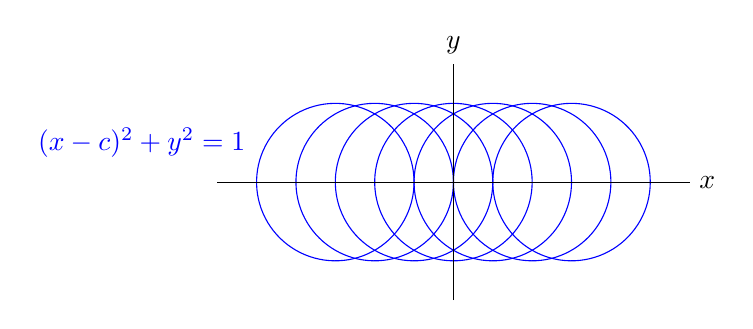
\begin{tikzpicture}[scale=1]
  % Curves
  \foreach \c in {-1.5,-1,...,1.5} {
    \draw[blue] plot[domain=0:2*pi, samples=100] ({\c + cos(\x r)}, {sin(\x r)});
  }
  % Labels
  \draw[-] (-3,0) -- (3,0) node[right] {$x$};
  \draw[-] (0,-1.5) -- (0,1.5) node[above] {$y$};
  \draw (-5.4,0.5) node[right,blue] {$(x-c)^2+y^2=1$};
\end{tikzpicture}$$
Derivando implícitamente, $2(x-c)+2y'y=0$, entonces $x-c=-yy'$. Sustitutyendo, tenemos que $(-yy')^2+y^2=1 \: \Rightarrow \: ((y')^2+1)y^2-1=0$, es decir, tenemos la ecuación implícita
$$F(x,y,p)=(p^2+1)y^2-1$$
Dado $q=(x_o,y_o)$, tenemos dos soluciones, ya que, despejando,
$$(p_o^2+1)y_o^2-1 = 0 \: \iff \: p_o= \pm \sqrt{\dfrac{1}{y_o^2}-1}$$
y tendremos que fijar alguna de las dos $p_o$ para asegurar la existencia y unicidad de las soluciones.
\end{eje}
\begin{obs}
    Como hemos visto en el ejercicio anterior, en ocasiones las soluciones no son únicas globalmente, por lo que tendremos que fijar un $p_o$ y tendremos soluciones en un entorno abierto suyo. 
\end{obs}
    Veamos algunas resoluciones de ecuaciones diferenciales especiales. 
    \begin{ejer}[\textbf{25.a}] $x=(y')^3-y'-1$
    \end{ejer}
    \begin{sol}
        Considerando $p=y'$ como parámetro, por la regla de la cadena,
        $$p=y'=\dfrac{dy}{dx}=\dfrac{\nicefrac{dy}{dp}}{\nicefrac{dx}{dp}}=\dfrac{\nicefrac{dy}{dx}}{3p^2-1} \; \Rightarrow \;  \dfrac{dy}{dp}=p(3p^2-1)$$
        por tanto, 
        $$y=\int (3p^3-p)dp=\dfrac{3}{4}p^4-\dfrac{p^2}{2}+c$$
        y las soluciones (parametrizadas) son 
        $$\left\{\begin{array}{l}
             x=p^3-p-1  \\
             y=\dfrac{3}{4}p^4-\dfrac{p^2}{2}+c
        \end{array}\right. \; c \in \mathbb R$$
    \end{sol}
    \begin{ejer}[\textbf{25.c}] $y=y' \log y'$
    \end{ejer}
    \begin{sol}
        $y=p \log p$
        haciendo la regla de la cadena,
        $$p=y'=\dfrac{dy}{dx}=\dfrac{\nicefrac{dy}{dp}}{\nicefrac{dx}{dp}}=\dfrac{\log p + 1}{\nicefrac{dx}{dp}} \; \Rightarrow \; \dfrac{dx}{dp}=\dfrac{1}{p} \log p + \dfrac{1}{p}$$
        y las soluciones por tanto
        $$\boxed{x=\dfrac{1}{2}\log^2 p + \log p + c}$$
    \end{sol}
    \begin{eje}[\textbf{25.f}] $y^{\nicefrac{2}{3}}+(y')^{\nicefrac{2}{3}}=1$
    \end{eje}
    \begin{sol}
        Dado que tenemos una suma de cuadrados igual a 1, tenemos relaciones trigonométricas, por tanto, haciendo el cambio de variable
        $$\left\{ \begin{array}{l}
             y^{\nicefrac{1}{3}}=\cos t  \\
             y'^{\nicefrac{1}{3}}=\sin t
        \end{array} \right. \; \Rightarrow \; \left\{ \begin{array}{l}
             y=\cos^3 t  \\
             y'=\sin^3 t
        \end{array} \right. \; \Rightarrow \; \sin^3 t= \dfrac{dy}{dx}=\dfrac{3\cos^2 t - \sin t}{\nicefrac{dx}{dt}}$$
    \end{sol}
\chapter{Sistemas de ecuaciones diferenciales ordinarias}
\section{Lineales de primer orden}
Llamaremos $y_1, \ldots, y_n$  las variables incógnitas y $t$ será la variable independiente. De esta forma, un sistema de ecuaciones diferenciales sería
$$\left\{ \begin{array}{c}
        \vspace{3mm} y'_1=\dfrac{dy_1}{dt}=f_1(y_1, \ldots, y_n)  \\
   y'_2=\dfrac{dy_2}{dt}=f_2(y_1, \ldots, y_n) \\
     \vdots \\
     y'_n=\dfrac{dy_n}{dt}=f_n(y_1, \ldots, y_n) 
\end{array} \right.$$
\begin{eje}\:
\begin{center}
        1. $\dfrac{dy}{dt}=y^2$ \qquad
        2. $\left\{ \begin{array}{l}
             \dfrac{dx}{dt}=x+y  \\
             \\
             \dfrac{dy}{dt}=\sin(xy) 
        \end{array} \right.$
\end{center}
\end{eje}
Veamos algunas resoluciones de ejercicios sencillos 
\begin{ejer}[\textbf{35.a}] Resolver el sistema
    $$\left\{ \begin{array}{ll}
         \frac{dx}{dt}=y  \\
         \frac{dy}{dt}=\dfrac{y^2}{x} 
    \end{array}\right.$$
\end{ejer}\begin{sol}
    Usando la regla de la cadena
    $$\dfrac{dy}{dt}=\dfrac{\nicefrac{dy}{dt}}{\nicefrac{dx}{dt}}=\dfrac{\nicefrac{y^2}{x}}{y}=\dfrac{y}{x}$$
    luego 
    $$\dfrac{dy}{y}-\dfrac{dx}{x}=0 \: \iff \: y=cx$$
    y sustituyendo en la 1ª ecuación tenemos que 
    $$\dfrac{dx}{dt}=cx \: \iff \: x=k\cdot e^{ct}$$
    y por tanto una solución es
    $$\left\{ \begin{array}{l}
         x=k \cdot e^{ct}  \\
         y=c\cdot k \cdot e^{ct} 
    \end{array}\right. \quad k,c \in \mathbb R$$
\end{sol}
\begin{defi}
    Dado el sistema, tenemos el campo vectorial asociado
    $$D=f_1(y_1, \ldots, y_n) \pd{}{y_1}+\cdots + f_n(y_1, \ldots, y_n)  \pd{}{y_n}$$
    llamamos \textbf{solución o curva integral} a cada curva parametrizada
    $$\begin{array}{rcl}
         \mathbb R \supseteq I & \overset{\Phi}{\longrightarrow} & U \subseteq \mathbb R^n  \\
         t & \longmapsto & \Phi(t):=(\Phi_1(t), \ldots, \Phi_n(t)) 
    \end{array}$$
    tal que 
    $$\Phi_{*,t_o}\left(\dfrac{d}{dt}\right)_{t_o}=\sum_{i=1}^n \left(\dfrac{d\Phi_i(t)}{dt} \right)_{t_o} \left(\pd{}{y_i} \right)_{\Phi(t_o)}=D_{\Phi(t_o)} \quad \forall \:  t_o \in I$$
    Es decir, $$\dfrac{d\Phi_i(t)}{dt}=f_i(\Phi_1(t), \ldots, \Phi_n(t))$$ es solución del sistema.
\end{defi}
\begin{ejer} \: 
    $\left\{ \begin{array}{l}
         \frac{dx}{dt}=-y  \\
         \frac{dy}{dt}=x
    \end{array}\right.$
\end{ejer}
\begin{sol}
    Haciendo como en el ejer. 35 la regla de la cadena, $x^2+y^2=c$. Por tanto
    $$y=\pm \sqrt{c^2-x^2} \: \Rightarrow \: \dfrac{dx}{dt}=\pm \sqrt{c^2-x^2} \: \Rightarrow \: \dfrac{dx}{\sqrt{c^2-x^2}} \; \Rightarrow \; \ldots \; \Rightarrow \; x=c_1 \:  \cos (t+c_2) , \: y=c_1 \: \sin (t+c_2) $$
\end{sol}
Veamos el siguiente importante ejemplo, ya que en situaciones genéricas, podemos convertir cualquier sistema en este por un cambio de coordenadas:
\begin{ejer} \: 
    $\left\{ \begin{array}{l}
         \frac{dx}{dt}=1  \\
         \frac{dy}{dt}=0
    \end{array}\right.$
\end{ejer}
\begin{sol}
    $$\left\{ \begin{array}{ll}
         \frac{dx}{dt}=1 \:& \Rightarrow \: x=t+c_1 \\
         \frac{dy}{dt}=0 \: &\Rightarrow \: y=c_2
    \end{array}\right.$$
\end{sol}
\section{Existencia y unicidad de soluciones}
Abreviando la notación, llamaremos 
$$Y:=\left( \begin{array}{c}
     y_1  \\
      y_2 \\
      \vdots \\
      y_n
\end{array}\right) \quad f(Y):=\left( \begin{array}{c}
     f_1(Y)  \\
      f_2(Y) \\
      \vdots \\
      f_n(Y) 
\end{array}\right)=\left( \begin{array}{c}
     f_1(y_1, \ldots, y_n)   \\
      f_2(y_1, \ldots, y_n)  \\
      \vdots \\
      f_n(y_1, \ldots, y_n)  
\end{array}\right)\quad Y':=\left( \begin{array}{c}
     y_1'  \\
      y_2' \\
      \vdots \\
      y_n'
\end{array}\right)$$
luego el sistema anterior se reduce a 
$$Y'=f(Y)$$
y de la misma forma, $Y=\Phi(t)$ es solución igual que antes.
\begin{prop}
    El problema de Cauchy
    $$\left\{\begin{array}{l}
         Y'=f(Y)  \\
         Y(t_o)=Y_o
    \end{array} \right. \quad Y_o \in \mathbb R^n$$
    con $f$ de Lipschitz: 
    $$\exists M \; / \; \|f\left(\overline{Y}\right)-f(Y)\|\leq M \|\overline{Y}-Y\|$$
    (por ejemplo si $f \in \mc{C}^1$ y soporte compacto, o $f \in \mc{C}^1$ y $\|df\|$ acotada)
    tiene como ecuación integral equivalente
    $$Y(t)=Y_o+\int_{t_o}^t f(Y(s)) \: ds$$
    y su solución existe y es única.
\end{prop}
\begin{dem}
    Definimos $I:=[t_o-\alpha, t_o+\alpha]$ y $E:=\mc{C}(I,\mathbb R^n)$. Sea $\phi: I \longrightarrow \mathbb R^n$, definimos en este espacio la norma 
    $$\|\phi\|=\sup_{t \in I} \|\phi(t)\|$$
    de forma que $(E, \|\cdot\|)$ es un espacio normado completo. Definiendo la trasnformación $T$ para adecuar los puntos fijos
    $$\begin{array}{rccccl}
        E & \overset{T}{\longrightarrow} & E  \\
        \phi & \longmapsto &  T \phi : & I & \longrightarrow & \mathbb R^n \\
         &&& t & \longmapsto &  \displaystyle (T \phi)(t):=Y(t)=Y_o+\int_{t_o}^t f(Y(s)) \: ds
    \end{array}$$
    de forma que $\phi$ es solución $\iff$ $T\phi=\phi$. Así pues, igual que en el caso en dos dimensiones \hyperref[demexuni]{\textit{Demostración Teorema de Existencia y Unicidad}}, con $\psi, \phi \in E$, tenemos que
    $$\|T\phi(t)-T\psi(t)\| \leq \alpha \cdot M \|\phi - \psi\|$$
    por tanto, si $\alpha \cdot M < 1$, $T$ es contractiva y tomando $\alpha < \nicefrac{1}{M}$ se termina la demostración. 
    \textbf{Ejercicio}: Demostrar la unicidad.
\end{dem}
\section{Sistemas autónomos y no autónomos}
Obsérvese la equivalencia del siguiente problema de Cauchy
$$\left\{\begin{array}{l}
     y'=f(x,y)  \\
     y(x_o)=y_o 
\end{array} \right. \iff \left\{\begin{array}{l}
     \dfrac{dx}{dt}=1  \\
     \vspace{-5mm} \\
     \dfrac{dy}{dt}=f(x,y) \\
     \vspace{-5mm} \\
     \hline x(x_o)=x_o \\
     y(x_o)=y_o
\end{array} \right.$$ donde la variable independiente $t$ no aparece en el primer miembro.
\begin{defi}
    Este tipo de sistemas de ecuaciones, en los que la variable independiente no aparece en los segundos miembro, son \textbf{sistemas autónomos}. En cambio, si aparace en ambos miembros, el sistema es \textbf{no autónomo}. Es decir, generalmente tendremos:
    $$\text{Autónomo } \left\{ \begin{array}{c}
        \vspace{3mm} y'_1=f_1(y_1, \ldots, y_n)  \\
   y'_2=f_2(y_1, \ldots, y_n) \\
     \vdots \\
     y'_n=f_n(y_1, \ldots, y_n) 
\end{array} \right. \quad 
\text{ No autónomo } \left\{ \begin{array}{c}
        \vspace{3mm} y'_1=f_1(t,y_1, \ldots, y_n)  \\
   y'_2=f_2(t,y_1, \ldots, y_n) \\
     \vdots \\
     y'_n=f_n(t,y_1, \ldots, y_n) 
\end{array} \right.$$
\end{defi}
\begin{cor}
    Por un simple cambio y ajuste de condiciones iniciales, cualquier problema no autónomo se convierte en autónomo.
\end{cor}
\begin{prop}
    Un problema autónomo tendrá soluciones si
    $$\|f(t,\overline{Y})-f(t,Y)\|\leq M\|\overline{Y}-Y\|$$
    es decir, $f$ es de Lipschitz en las variables dependientes.
\end{prop}
\begin{ejer}[\textbf{34}]
     $\left\{ \begin{array}{l}
        \frac{dx}{dt}=x \\
        \frac{dy}{dt}=t y 
\end{array} \right.$
\end{ejer}
\begin{sol}
     $$\left\{ \begin{array}{l}
        \frac{dx}{dt}=x \; \Rightarrow \; x=c_1 e^t\\
        \frac{dy}{dt}=t y \; \Rightarrow \; \dfrac{dy}{y}=t dt \; \Rightarrow \; \log|y|-\nicefrac{t^2}{2}=k \; \Rightarrow \; y=c_2e^{\nicefrac{t^2}{2}}
\end{array} \right.$$
\end{sol}
\begin{ejer}
 $\left\{ \begin{array}{l}
        \frac{dx}{dt}=x \\
        \frac{dy}{dt}=t x 
\end{array} \right.$
\end{ejer}
\begin{sol}
    $$\left\{ \begin{array}{l}
        \frac{dx}{dt}=x \; \Rightarrow \; x=c_1 e^t \\
        \frac{dy}{dt}=t x = tc_1e^t \; \Rightarrow \; y=c_1 \int t e^t dt + c_1
\end{array} \right.$$
\end{sol}
\section{Sistemas lineales}
Son sistemas de la forma
$$\left\{ \begin{array}{l}
        \vspace{3mm} \dfrac{dy_1}{dt}= a_{11}(t)y_1+\cdots+ a_{1n}(t)y_n + b_1(t) \\
        \dfrac{dy_2}{dt}= a_{21}(t)y_1+\cdots +a_{2n}(t)y_n + b_2(t) \\
      \quad \vdots \\
     \dfrac{dy_n}{dt}= a_{n1}(t)y_1+\cdots +a_{nn}(t)y_n + b_n(t)
\end{array} \right.$$
que de forma matricial es
$$Y'=A(t)Y + B(t)=f(t,Y)$$
y cuando $B=\Big( 0 \Big)$ se dice que es un sistema homogéneo y si $B\neq \Big( 0 \Big)$ se llama sistema lineal completo.
\subsection{Espacio de soluciones}
Sea $t \in I$ un intervalo abierto de $\mathbb R$, se tiene que las matrices $A(t)$ y $B(t)$ son las aplicaciones
$$\begin{array}{rcl}
     \mathbb R \supseteq I & \overset{A}{\longrightarrow} & M_{n \times n}(\mathbb R) \\
     I & \overset{B}{\longrightarrow} & \mathbb R^n 
\end{array}$$
Sea $J \subset I$ un compacto, veamos que en él, $f$ es de Lipschitz:
$$\|f(t,\overline{Y})-f(t,Y)\| = \|A(t) (\overline{Y}-Y)\|\leq \|A(t)\|\|\overline{Y}-Y\| \leq \left(\max_{t \in J}\|A(t)\|\right) \|\overline{Y}-Y\| \leq M_J \|\overline{Y}-Y\|$$
asegurando la existencia de $M_J$ por ser $J$ compacto, de forma cualquier función alcanza su mínimo y su máximo. Al igual que en problema en dos variables, se puede ampliar $J$ (hasta donde se quiera) siendo $M_J$ una constante global, y por tanto encontrando una solución global.

Así que la única condición necesaria es que $a_{ij}$ y $b_j$ sean lineales.

\subsection{Estructura del espacio de soluciones}
\underline{Caso homogéneo}

Dadas dos soluciones, $Y_1'=AY_1$ y $Y_2'=AY_2$ de forma que la suma $(Y_1+Y_2)'=A(Y_1+Y_2)$ es también solución, y $(\lambda Y_1)'=A \lambda Y_1$ también. De esta forma, 
$$\left\{\begin{array}{c}
     \text{Soluciones de }  \\
     Y'=AY
\end{array} \right\}=\text{ Espacio vectorial sobre } \mathbb R$$
Veamos cual es su dimensión. Consideremos, para cada $i = 1, \: \ldots, \: n$ la solución (única) $Y_i$ del problema de Cauchy:
$$\left\{\begin{array}{l}
     Y'=A(t) Y  \\
     Y(t_o)=(0, \ldots, 0, 1, 0, \ldots, 0) \quad (\text{un 1 en lugar }i\text{-ésimo}).
\end{array} \right.$$
Las soluciones $Y_i$ son sistema de generadores, ya que si $Y$ es una solución arbitraria tal que $Y(t_o)=(\lambda_1, \ldots, \lambda_n)$, entonces $\displaystyle Y=\sum_i \lambda_i Y_i$. Por otra parte, las soluciones $Y_1, \ldots, Y_n$ son linealmente independientes, ya que si tenemos $$\sum_i \mu_i Y_i= 0 \; \Rightarrow \; (\mu_1,\ldots, \mu_n)=\left( \sum_i \mu_i Y_i \right)(t_o)=0$$
por tanto, $Y_i \in \mathbb R^n$ son base y por tanto su dimensión es $n$.
\begin{cor}
    Toda solución $Y$ es de la forma $Y=c_1 Y_1 + c_2 Y_2 + \cdots + c_n Y_n$ con $c_1, \ldots, c_n \in \mathbb R$.
\end{cor}
\begin{defi}
 La base del espacio de soluciones, $Y_1, \ldots, Y_n$ se denomina \textbf{sistema fundamental de soluciones}.
\end{defi}

Definiendo la matriz 
$$W:=\Big( Y_1 \:  | \:  Y_2 \: | \: \cdots \: | \:  Y_n \Big), \; C=\left(\begin{array}{c}
     c_1  \\
     \vdots \\
     c_n
\end{array}\right)$$
tenemos que las soluciones son 
$$\boxed{Y=W \cdot C}$$
\begin{defi}
    La matriz $W:=\Big( Y_1 \:  | \:  Y_2 \: | \: \cdots \: | \:  Y_n \Big)$ poniendo las soluciones como columnas la denominamos Wronskiano. Podemos ver una representación gráfica:
    \begin{figure}[h]
        \centering
        \includegraphics[scale=0.6]{wronskiano.png}
        \label{fig:wronskiano}
    \end{figure}

\end{defi}
\underline{Caso completo}

Dado que la resta de soluciones de $Y'=AY+B$ es solución de la homogénea, sean $Y_1, Y_2$, entonces $Y_1-Y_2$ es solución de la homogénea. Así pues, toda solución es 
$$Y=Y_p+Y_h$$
entonces 
$$\left\{\begin{array}{c}
     \text{Soluciones de }  \\
     Y'=AY+B
\end{array} \right\}=Y_p+\left\{\begin{array}{c}
     \text{Soluciones de }  \\
     Y'=AY
\end{array} \right\}=\text{ Espacio afín}$$

\subsection{Sistemas homogéneos}
Sea $A \in M_{n \times n}(\mathbb R)$, consideremos el sistema $Y'=AY$. Considerando la matriz $e^{tA}$, que además verifica que $(e^{tA})'=A e^{tA}$, tenemos que dado $Y:=e^{tA} \: C$,
$$Y'=(e^{tA} \: C)'=(e^{tA})'C=A e^{tA} C=AY$$

Así pues
$$e^{tA} \begin{pmatrix}
1  \\
0 \\ \vdots \\ 0 
\end{pmatrix}, \; e^{tA} \begin{pmatrix}
0  \\
1 \\ \vdots \\ 0 
\end{pmatrix}, \: \ldots , \:e^{tA} \begin{pmatrix}
0  \\
\vdots \\ 
0 \\
1 
\end{pmatrix}$$
son base de las soluciones, teniendosé el homeomorfismo
$$\begin{array}{rcl}
     \mathbb R^n & \longrightarrow & Soluciones  \\
     C & \longmapsto & e^{tA} \: C 
\end{array}$$
\textbf{Observación}. En cambio, $Z:=C e^{tA}$ no es solución ya que 
$$Z'=(C e^{tA})'=C (e^{tA})'=C \:  A \: e^{tA}$$
\begin{propi} \: 
\begin{enumerate}
    \item $e^{(t+s)A}=e^{tA} \cdot e^{sA}$
    \item $e^{0 A}=Id$
    \item $(e^{tA})^{-1}=e^{-tA}$
\end{enumerate}
\end{propi}

\subsection{Método de variación de las constantes}
La función de este apartado es el cálculo de una solución particular partiendo de un sistema fundamental de soluciones de la homogénea.

Sean $\Phi_1, \: \ldots, \: \Phi_n$ una base de soluciones de {\scriptsize $\left\{\begin{array}{c}
     \text{Soluciones de}  \\
     Y'=AY
\end{array} \right\}$}, entonces $Y_h=W \cdot C$. Entonces buscamos una solución $Y_p$ de $Y'=AY+B$ que tenga la forma $Y_p=W \cdot C(t)$, es decir verifica ambas ecuaciones:
$$Y'_p=AY_p+B=AWC(t)+B \quad Y'_p=(W C(t))'=W'C+WC'=AWC+WC'$$
donde $W'=A \cdot W$ por ser $W$ soluciones y verificar la ecuación diferencial, y por tanto, 
$$AWC+B=AWC+WC' \; \iff \; B=W \cdot C' \; \iff \; C'=W^{-1} \cdot B \; \iff \; C(t)=\int W^{-1}\cdot B \: dt$$
\begin{obs}
 $W$ siempre es invertible. Supongamos que $det \: W $ se anula para cierto $t_o$, entonces existe $\lambda_1, \ldots, \lambda_n$ tal que $\lambda_1 \Phi_1(t_o)+ \cdots + \lambda_n \Phi_n(t_o)=0$. Sea $\Phi:=\lambda_1 \Phi_1+ \cdots + \lambda_n \Phi_n$, entonces $\Phi$ es solución de 
 $$\left\{ \begin{array}{l}
      Y'=AY  \\
      Y(t_o)=0 
 \end{array}\right.$$
 pero la existencia de la solución $Y=0$ asegura que la única solución es esa, por lo que $\Phi=0$ es idénticamente 0, y por tanto $\Phi_1, \: \ldots , \: \Phi_n$ son linealmente dependientes, así pues no son base, llegando a una contradicción y por tanto $det \: W \neq 0 \: \forall t \in \mathbb R$.  
\end{obs}
\subsection{Problema de Cauhy}
Consideremos el problema de Cauchy
$$\left\{ \begin{array}{l}
     Y'=AY  \\
     Y(0)=P 
\end{array}\right. \; \Rightarrow \; \left\{ \begin{array}{l}
     Y=e^{tA}C  \\
     Y(0)=P 
\end{array}\right. \; \Rightarrow \; \left\{ \begin{array}{l}
     Y=e^{tA}C  \\
     P =Y(0)= e^{0A}C=Id \cdot C=C
\end{array}\right.$$
es decir, la condición inicial nos muestra el vector de constantes.
\begin{obs}
    Así pues, considerando el conjunto $\{e^{tA}\}_{t \in \mathbb R}$ es un grupo 1-paramétrico de transformaciones (lineales) de $\mathbb R^n$, ya que $e^{tA}\in L(\mathbb R^n, \mathbb R^n)$.
\end{obs}
\begin{prop} Por lo ya visto, $e^{tA}$ (con $A$ cte.) es la única solución (ejercicio trivial) de 
    $$\left\{ \begin{array}{cc}
         W'=AW  \\
         W(0)=I 
    \end{array} \right.$$
\end{prop}
\begin{prop}
    Generalizando ahora, consideramos $A(t)$, se tiene el problema de Cauchy
    $$(*)\left\{ \begin{array}{l}
         S'=A(t)S, \qquad S(t)\in M_{n \times n}(\mathbb R)  \\
         S(t_o)=I 
    \end{array} \right.$$
    A la solución de $(*)$ la denotamos por $S(t,t_o)$
\end{prop}
Por tanto, 
$$\text{la solución de }\left\{ \begin{array}{l}
         Y'=A(t)Y   \\
         Y(t_o)=Y_o 
    \end{array} \right. \text{ es } Y=S(t,t_o)Y_o$$
    En efecto:
    $$Y'=(S(t,t_o)\cdot Y_o)'=S(t,t_o)' \cdot Y_o = A(t)\cdot S(t,t_o) \cdot Y_o =A(t)\cdot Y$$
    $$Y(t_o)=S(t_o,t_o)\cdot Y_o=I \cdot Y_o = Y_o$$ 
    \;
    \begin{eje}
    Si $A$ es constante, $S(t,t_o)=e^{(t-t_o)A}$
\end{eje}
    \begin{propi} \: 
        \begin{enumerate}
            \item $S(t_o,t_o)=Id$
            \item $S(t,t_o)=S(t,t_1)S(t_1,t_o)$
            \begin{dem}
                $S(t,t_o)$ es solución de $(*)$, $S(t,t_1)$ poniendo $t_1$ donde $t_o$, probemos pues si $S(t,t_1)S(t_1,t_o)$ es solución de un problema de valor inicial. En efecto
                $$(S(t,t_1)S(t_1,t_o))'=S(t,t_1)'S(t_1,t_o)=A(t) (S(t,t_1) S(t_1,t_o))$$
                verificando la ecuación (1) de $(*)$. Veamos si verifica la de valor inicial:
                $$S(t_1,t_1)S(t_1,t_o)=S(t_1,t_o)$$
                por tanto, $S(t,t_1) S(t_1,t_o)$ es solución de 
                $$\left\{ \begin{array}{l}
                     S'=AS  \\
                     S(t_1)=S(t_1,t_o) 
                \end{array} \right.$$
                pero 
                $$\left\{ \begin{array}{l}
                     S(t,t_o)'=AS(t,t_o)  \\
                     S(t_1,t_o)=S(t_1,t_o) 
                \end{array} \right.$$
                luego por unicidad, 
                $$S(t,t_1) S(t_1,t_o)=S(t,t_o)$$
            \end{dem}
            \item $S(t_1,t_o)=S(t_o,t_1)^{-1}$
            \begin{dem}
                Usando la propiedad anterior, con $t=t_o$ se demuestra.
            \end{dem}
            \item Si $\Phi_1, \: \ldots, \Phi_n$ son base de soluciones de $Y'=AY$, el wronskiano $W:=\Big( \Phi_1 \: | \: \cdots \: | \:  \Phi_n \Big)$ verifica que $W'=AW$, luego 
            $$S(t,t_o)=W(t) W(t_o)^{-1}$$
        \end{enumerate}
    \end{propi}
    \subsection{Fórmula de Duhamel}
    Sea el sistema 
    $$\left\{\begin{array}{l}
                Y'=A(t)Y+B(t)  \\
                Y(t_o)=Y_o 
             \end{array} \right.$$
             con $S(t,t_o)$ conocida, entonces llamando $Y:=S(t,t_o) \overline{Y}$ (luego $\overline{Y}:=S(t,t_o)^{-1}Y$) y $B=S(t,t_o) \overline{B}$ ($\overline{B}=S(t,t_o)^{-1}B$) luego podemos reescribir el problema como 
    $$\left\{\begin{array}{l}
                Y'=(S(t,t_o)^{-1} \overline{Y})'=S(t,t_o)' \overline{Y} + S(t,t_o)\overline{Y}'=AS(t,t_o) \overline{Y} +S(t,t_o) \overline{Y}' \\
                ||\\
                AY+B=AS(t,t_o)\overline{Y}+S(t,t_o)\overline{B}
             \end{array} \right.$$
             pudiendo eliminar de todos los miembros $S(t,t_o)$ (por tener inversa) y obteniendo que $$\overline{Y}'=\overline{B}$$
             Veamos que verifica la misma condición inicial:
             $$Y(t_o)=S(t_o,t_o)\overline{Y}(t_o)=I\overline{Y}(t_o)=\overline{Y}(t_o)$$
             y por tanto $\overline{Y}$ es la solución de 
             $$\left\{ \begin{array}{l}
                  \overline{Y}'=\overline{B}  \\
                  \overline{Y}(t_o)=Y_o                  
             \end{array} \right.$$
             Es decir, 
             $$\overline{Y}=Y_o+\int_{t_o}^t \overline{B}(s)ds$$
             por tanto, deshaciendo el cambio de variable,
             $$S(t,t_o)^{-1}Y(t)=Y_o+\int_{t_o}^t S(s,t_o)^{-1} B(s) ds \; \iff \; Y(t)=S(t,t_o)Y_o+S(t,t_o) \int_{t_o}^t S(s,t_o)^{-1} B(s) ds $$
             $$ \; \underset{3.}{\overset{2.}{\iff}} \; \boxed{Y(t)=S(t,t_o)Y_o+\int_{t_o}^t S(t,s) B(s) ds \; } \qquad \text{Fórmula de Duhamel}$$
             
             Con las notaciones precedentes, se tiene el siguiente
\begin{lem} 
    Si $\|A(t)\| \leq M$ para todo $t$, entonces \label{lema4.4}
    $$\|S(t,t_o)\| \leq e^{M|t-t_o|}$$
    con la norma del supremo en matrices:
    $$\|B\|=\sup_{\|v\|\leq 1}\|B(v)\| \qquad B \in M_{n \times n}(\mathbb R) , \; v \in \mathbb R^n $$
    \end{lem}
\begin{dem}
Se puede reducir al caso $t_o=0$ considerando como nueva variable independiente a $t - t_o$. Por otro lado, basta hacer la demostración para $t \geq 0$ cambiando $A(t)$ por $-A(-t)$ cuando $t$ sea negativa. Definimos el vector $z(t):=e^{-Mt} \: S(t,0) \: v$ con $v \in \mathbb R^n$. Si probamos que $\|z\| \leq \|v\| \; \forall v \in \mathbb R^n$, entonces sería $\|e^{-Mt} \: S(t,0) \| \leq 1$ y despejando terminaríamos.

Definiendo $\varphi(t):=\|z\|^{2}=(z,z)$ al producto escalar (obs.: $\varphi(0)=\|v\|^2$) veamos que no crece, es decir, decrece. Derivando $z$
$$z'=(e^{-Mt} \: S(t,0) \: v)'=(e^{-Mt})' \: S(t,0) \: v + e^{-Mt} \: S(t,0)' \: v= $$ 
$$= -Me^{Mt} \: S(t,0) \: v + e^{-Mt} \: A(t) \: S(t,0) \: v = (A(t)-M) z$$
y derivado $\varphi$ y sustituyendo
$$\varphi'(t)=(z,z)'=2(z',z) \; \Rightarrow \; z'=2((A(t)-M)z,z) \overset{(1)}{\leq} 0$$
luego la derivada es negativa y por tanto la función $\varphi$ es no creciente, luego $\varphi(t) \leq \varphi(0)$ para todo $t \geq 0$.

$^{(1)} (A(t)z,z) \leq \|A(t)z\|\cdot \|z\| \leq \|A(t)\|\cdot \|z\|\cdot \|z\| \leq M \cdot \|z\|^2 = (Mz,z)$
     \end{dem}

\chapter{Ecuaciones diferenciales ordinarias de orden superior}

Son ecuaciones de la forma $$\: \: (*)\: \: \boxed{\: y''=f(x,y,y') \: } $$ y para su resolución usamos $y_o:=y$ e $y_1:=y'$, de forma que tenemos las ecuaciones
$$(**)\left\{ \begin{array}{l}
     y_o'=y_1  \\
     y_1'=f(x,y_o,y_1) 
\end{array} \right.$$
\begin{prop}
    $(*)$ y $(**)$ son equivalentes
\end{prop}
\begin{dem}
    Que sean equivalentes significa que tienen las mismas soluciones. Supongamos que $y=\phi(x)$ es solución de $(*)$, entonces 
$$\begin{pmatrix}
    y_o \\ y_1
\end{pmatrix}=\begin{pmatrix}
    \phi(x) \\ \phi'(x)
\end{pmatrix}$$ es solución de $(**)$.

Recíprocamente, si
$$\begin{pmatrix}
    y_o \\ y_1
\end{pmatrix}=\begin{pmatrix}
    \psi_o(x) \\ \psi_1(x)
\end{pmatrix}$$
es solución de $(**)$, entonces $y_o=\psi_o(x)$ es solución de $(*)$.
\end{dem}
\begin{obs}
    Reiteradamente, se pueden resolver ecuaciones de orden mayor que 2, así que podemos usar todo los conocimientos de sistemas ecuaciones ordinarias, pudiendo también asegurar la existencia y unicidad de soluciones.
\end{obs}
\begin{eje}
    Sea la ecuación lineal (en las $y$'es) $y''=a_o(x)y+a_1(x)y'+b(x)$, su sistema asociado es
    $$\left\{ \begin{array}{l}
     y_o'=y_1  \\
     y_1'=a_o(x)y_o+a_1(x)y_1+b(x) 
\end{array} \right. \longleadsto{1} \begin{pmatrix}
    y_o \\ y_1
\end{pmatrix}'=\begin{pmatrix}
    0 & 1 \\
    a_o(x)& a_1(x)
\end{pmatrix} \begin{pmatrix}
    y_o \\ y_1 
\end{pmatrix}+\begin{pmatrix}
    0 \\ b(x)
\end{pmatrix}$$
\end{eje}

\section{Solución de ecuaciones por desarrollo en series de potencias}

\begin{prop}
    Sea la serie de potencias
    $$S(x)=\sum_{n=0}^{\infty} a_n (x-x_o)^n$$
    \begin{enumerate}
        \item Existe $R$ tal que $S$ converge absolutamente en $|x-x_o| < R$. 
        \item En $|x-x_o|> R$ diverge.
        \item En $|x-x_o|=R$ pueden ocurrir las dos posibilidades.
    \end{enumerate}
\end{prop}
\begin{defi}
    A $R$ lo llamamos \textbf{radio de convergencia}
\end{defi}
\begin{prop}
    Si 
    $$\lim_{n \to \infty} \sqrt[n]{|a_n|}=L \; \; \; \left(ó \lim_{n \to \infty}\left| \dfrac{a_{n+1}}{a_n}\right|=L \right) \; \Rightarrow \; R=\dfrac{1}{L}$$
\end{prop}
\begin{propi}
Si $\displaystyle S(x)=\sum a_n(x-x_o)^n$ y $\displaystyle T(x)=\sum b_n(x-x_o)^n$ convergen en $(x_o-R, \: x_o+R)$, entonces
$$S(x)+T(x)=\sum_{n=0}^{\infty} (a_n+b_n)(x-x_o)^n \qquad S(x) \cdot T(x)=\sum_{n=0}^{\infty} \left(\sum_{i+j=n} a_ib_j\right)(x-x_o)^n$$
de la misma forma, podemos definir la derivada
$$S'(x)=\sum_{n=1}^{\infty}n \: a_n (x-x_o)^{n-1}$$
y como podemos derivar las veces que queramos, se tiene que $S \in \mc{C}^{\infty}$.
\end{propi}
\begin{defi}
Sea $\mathbb R \supset I \overset{f}{\longrightarrow} \mathbb R$ de clase $\mc{C}^{\infty}$, diremos que $f$ es \textbf{analítica} si $\forall x_o$ , $f$ coincide con $S(x)$ en un entorno de $x_o$. 
\end{defi}
\begin{prop}
    La única opción además es que $S(x)$ sea su desarrollo en serie de Taylor coincide con la función.
\end{prop}
\begin{dem}
    Si $f(x)=\sum b_n(x-x_o)^n=b_o+b_1(x-x_o)+b_2(x-x_o)+\cdots$
    entonces $f'(x)=b_1+2b_2(x-x_o)+\cdots $, $f''(x)=2b_2+3b_3(x-x_o)$, de forma que $$b_o=f(x_o), \quad b_1=f'(x_o), \quad 2b_2=f''(x_o), \: \ldots \: , \quad b_n=\frac{f^{(n}(x_o)}{n!} $$ teniéndose así que la serie es el desarrollo de Taylor.
\end{dem}
\begin{obs}
    Aunque parezca tautología, las series de potencias son analíticas, esto es coinciden con la serie también en un entorno de $x_o$, por ejemplo, si $p \in (x_o-R, \: x_o+R)$, $S(x)=\sum b_n(x-p)^n$
\end{obs}
\begin{ejes}
Veamos algunos ejemplos de funciones analíticas:
\begin{enumerate}
    \item $f(x)=e^x=\mathlarger{\sum} \frac{x^n}{n!} \quad R=+\infty$
    \item $F(x)=\log(1+x) \quad R=1$
    \item La función \vspace{-20mm}
    \begin{multicols}{3}[\columnsep=5mm]
    \subsection*{}
    $$h(x)=\left\{\begin{array}{ll}
    \; e^{-\nicefrac{1}{x^2}} & \text{ si } x \neq 0 \\ \; 0 & \text{ si } x =0
    \end{array}\right.$$ \columnbreak
    \subsection*{}
    \begin{tikzpicture}[scale=0.6]
    \begin{axis}[
    axis lines=middle,
    xmin=-3,xmax=3,
    ymin=-0.5,ymax=1.5, 
    tick align=outside,
    xtick={-3,-2,-1,0,1,2,3},
    ytick={0,0.5,1},
    domain=-3:3,
    samples=200
    ]
    \addplot [red] {exp(-1/(x^2))} node[above left] {$h(x)$};
    \end{axis}
    \end{tikzpicture}
    \subsection*{}
    \begin{tikzpicture}[scale=0.6]
    \begin{axis}[
    axis lines=middle,
    xmin=-1,xmax=1,
    ymin=-0.5,ymax=1.5, 
    tick align=outside,
    xtick={-1,-0.5,0,0.5,1},
    ytick={0,0.5,1},
    domain=-1:1,
    samples=100
    ]
    \addplot [red] {exp(-1/(x^2))} node[above left] {$h(x)$};
    \end{axis}
    \end{tikzpicture}
    \end{multicols}
    es de clase $\mc{C}^{\infty}$ y además $h^{(n)}(0)=0$ (como vemos en el gráfico, es practicamente 0 entorno al 0), de forma que la serie de Taylor es $S(x)=0$ idénticamente nula, así pues no es analítica.
\end{enumerate}
\end{ejes}
\begin{defi}
    Sea $S(x)$ y $T(x)$ dos series definidas como antes, diremos que $T(x)$ es mayorante de $S(x)$ si $|a_n|\leq |b_n|$. 
\end{defi}
\begin{prop}
    Si $T(x)$ es mayorante de $S(x)$, donde converge $T(x)$, converge $S(x)$, es decir, que $R_{S(x)} \geq R_{T(x)}$.
\end{prop}
\begin{cor}
Esta proposición es de gran utilidad ya que podremos usar series fáciles para acotar series más complejas.
\end{cor}

\begin{lem}
    Cosideremos la ecuación $$y''=\dfrac{M}{1-\frac{x}{r}}(y'+y)$$
    tal que $M,r \in \mathbb R^+$ y $Mr > 2$ y se trata de econtrar soluciones analíticas de la forma $\displaystyle y=\sum_{n=0}^{\infty} b_n \: x^n$, es decir, encontrar las $b_n$. 
\end{lem}
\begin{dem}
    Modificando la ecuación:
    $$0=\left(1-\dfrac{x}{r}\right) y''-My'+My=$$
    $$=\sum_{n=0}^{\infty} (n+2)(n+1)b_{n+2} \: x^n - \sum_{n=1}^{\infty} \dfrac{(n+1)n}{r} \: b_{n+1} \:  x^n - M \sum_{n=0}^{\infty} (n+1) \: b_{n+1} x^n- M \sum_{n=0}^{\infty} b_n \: x^n=$$
    $$=2b_2-Mb_1-Mb_o+\mathlarger{\sum_{n=0}^{\infty}}\left( (n+2)(n+1)\: b_{n+2} - \left(\dfrac{(n+1)n}{r}+M(n+1) \right)b_{n+1}-M\: b_n\right) \: x^n=0 \iff$$
    $$\iff \begin{cases}
        0=2b_2-Mb_1-Mb_o \\
        0=(n+2)(n+1)\: b_{n+2} - \left(\dfrac{(n+1)n}{r}+M(n+1) \right)b_{n+1}-M\: b_n
    \end{cases}$$
    de forma que obtenemos la ecuación general
    $$b_{n+2}=\dfrac{1}{r} \cdot \dfrac{n+Mr}{n+2} \: b_{n+1} + \dfrac{M}{(n+1)(n+2)} \: b_n$$
    Dada esta expresión es difícil obtener $b_n$ como una función de $b_o$ y $b_1$, pero podemos demostrar que $\sum b_n \: x^n$ es convergente cuando $|x|<r$. 

    Volviendo a la expresión de $b_{n+2}$, dada la hipótesis de $Mr>2$, $$b_{n+2}>\dfrac{b_{n+1}}{r} \; \iff \; \dfrac{b_{n+1}}{b_{n+2}}<r$$
    Dividiendo dos términos consecutivos de la expresión:
    $$\dfrac{b_{n+2}}{b_{n+1}}=\dfrac{1}{r} \cdot \dfrac{n+Mr}{n+2}+\dfrac{M}{(n+1)(n+2)} \cdot \dfrac{b_n}{b_{n+1}}$$
    y haciendo límite,
    $$\lim_{n \to \infty} \dfrac{b_{n+2}}{b_{n+1}}=\lim_{n \to \infty} \dfrac{1}{r} \cdot \dfrac{n+Mr}{n+2}+\cancelto{0}{\dfrac{M}{(n+1)(n+2)}} \cdot \dfrac{b_n}{b_{n+1}} = \dfrac{1}{r}$$
    ya que $ \frac{b_n}{b_{n+1}}$ está acotado, como acabábamos de ver.

    De esta forma, hemos demostrado que la serie converge y que el radio de convergencia es $R=\dfrac{1}{\nicefrac{1}{r}}=r$.
\end{dem}
\begin{teo}
 Sean $P(x)$ y $Q(x)$ análiticas convergentes en $|x-x_o|<R$. Entonces las soluciones de $$y''=P(x)y'+Q(x)y$$
 son analíticas en un entorno de $x_o$ y convergen en $|x-x_o|<R$.
\end{teo}
\begin{dem}
    Supongamos que $x_o=0$ y denotemos $\displaystyle P(x)=\sum_{n=0}^{\infty} p_n \: x^n$ y $\displaystyle Q(x)=\sum_{n=0}^{\infty} q_n \: x^n$ convergetes en $|x|<R$. Sea $r \in (-R,R)$, entonces las series $\sum p_n \: r^n $ y $\sum q_n \: r^n$ son convergentes (son series de números con un $r$ dentro del radio de convergencia) y además, el término general de ambas tiende a 0 ya que convergen, por tanto
    $$\exists M>0 \text{ tal que } \begin{cases}
        |p_n| \: r^n <M \\ |q_n| \: r^n <M
    \end{cases} \: \forall n$$
    teniéndose las series
    $$|p_n| < \dfrac{M}{r^n} \qquad   |q_n| < \dfrac{M}{r^n} $$
    y además, la serie (geométrica) $$\sum \dfrac{M}{r^n} \: x^n = M \sum \left( \dfrac{x}{r}\right)^n=M \cdot \dfrac{1}{1-\frac{x}{r}}$$ es mayorante de las anteriores.

    Haciendo la derivada de la serie de $y$,
    $$y''=P(x)y'+Q(x)y=$$
    $$=(p_o+p_1xp_2x^2+\cdots)(a_1+2a_2x+3a_3x^2+\cdots)+(q_o+q_1x+q_2x^2+\cdots )(a_o+a_1x+a_2x^2+\cdots )$$
    y obtenidas las relaciones de recurrencia, deduciremos que 
    $$a_k=A_{k_o}(p,q) \: a_o + A_{k_1}(p,q) \: a_1$$
    donde $A_{k_o}, A_{k_1}$ son polinomios en las $p'$s y las $q'$s de coeficientes no negativos $^{(1)}$. Como además no dependen de la expresión concreta, hemos obtenido una fórmula \underline{universal}, es decir, que conociendo $a_o$ y $a_1$ deducimos todos los $a_k$. Si demostramos que $\sum a_n \: x^n $ converge habremos terminado.

    Consideramos los dos problemas de Cauchy:
    $$\left\{ \begin{array}{l}
         y''=P(x)y'+Q(x)y \\
        a_o,a_1         
    \end{array}\right. \qquad \left\{ \begin{array}{l}
         y''=\dfrac{M}{1-\frac{x}{r}}\: y'+ \dfrac{M}{1-\frac{x}{r}} \: y  \\
          b_o=|a_o|, b_1=|a_1| \\
    \end{array}\right.$$
    donde las soluciones de la segunda son $y= \sum b_n \: x^n$ tal que 
    $$b_k=A_{k_o}(\overline{p}, \overline{q})b_o+A_{k_1}(\overline{p}, \overline{q})b_1$$
    y por tanto se verifica que 
    $$|a_k| \leq \underbrace{A_{k_o}(|p|,|q|)}_{\leq^{(1)} A_{k_o}(\overline{p}, \overline{q})} \: |a_o| + \underbrace{A_{k_1}(|p|,|q|)}_{\leq^{(1)} A_{k_1}(\overline{p}, \overline{q})}\: |a_1| \leq b_k$$
    ($^{(1)}$ por ser de coeficientes o negativos) y por tanto $\sum b_n \: x^n$ es mayorante de $\sum a_n \: x^n$. Y como $\sum b_n \: x^n$ converge en $|x|<r$ (como hemos visto en el ejemplo anterior), entonces $\sum a_n \: x^n$ también converge. \hfill $\blacksquare$.
\end{dem}
\section{Dependencia de las condiciones iniciales}

Sea el problema de Cauchy del sistema de ecuaciones diferenciales:
$$\left\{ \begin{array}{l}
     Y'=f(Y)  \\
     Y(t_o)=Y_o
\end{array}\right.$$
entonces, por el Teorema de Existencia y Unicidad, fijando un intervalo, existe una única solución verificando el problema. Esta sección trata de hallar qué sucede si cambiamos la condición inicial $Y_o$. 
\begin{teo}[\textbf{de dependencia continua respecto de las condiciones iniciales}]
Considerando la solución $Y(t,Y_o)$, intuitivamente, si cambiamos ligeramente la condición inicial, la solución varía ligeramente, por lo que la depencia de $Y$ es continua respecto de $Y_o$.
\end{teo}
\begin{dem}
    Cambiemos la notación y llamemos $\lambda=Y_o$ y demostraremos que $Y(t,\lambda)$ es continua. La idea de la demostración es la misma que para existencia y unicidad, demostrado la contractividad de $Y(t,\lambda)$ respecto de $t$ y de $\lambda$. 

    Sea $I=[t_o-\alpha, t_o+\alpha]$ y sea $\Lambda$ un paralelepípedo cerrado en $\mathbb R^n$ tal que $\lambda \in \Lambda$. Definimos la aplicación
    $$\begin{array}{rcl}
         I \times \Lambda & \overset{\Phi}{\longrightarrow} & \mathbb R^n  \\
         (t, \lambda) & \longmapsto & \Phi(t,\lambda) 
    \end{array}$$
    y en el conjunto de todas esas aplicaciones (y continuas), , que es el conjunto $E:=\mc{C}(I \times \Lambda, \mathbb R^n)$, buscaremos las soluciones. Elegimos en él la norma 
    $$\|\Phi\|=\sup_{(t,\lambda) \in I \times \Lambda}\|\Phi(t,\lambda)\|_{\mathbb R^n}$$
    teniéndose así el espacio $(E,\|\cdot\|)$ normado completo, i.e. de Banach. 

    Definimos la aplicación contractiva $T: E \longrightarrow E$, igual que en el teorema de existencia y unicidad:
    $$(T\Phi)(t,\lambda)=\lambda + \int_{t_o}^t f(\Phi(s,\lambda))ds$$
    y como es contractiva y $(E, \|\cdot \|)$ es de Banach, hay un punto fijo, y sea la solución $Y(t,\lambda) \in \mc{C}(I \times \Lambda, \mathbb R^n)$, entonces 
    $$Y(t,\lambda )=\lambda + \int_{t_o}^t f(Y(s, \lambda)) ds$$
    y por tanto se demuestra la continuidad de la solución, por pertenecer a $E$.
\end{dem}
\section{Dependencia respecto de parámetros}
Consideremos la familia de ecuaciones definidas por el parámetro $\mu$
$$\left\{ \begin{array}{l}
     y'=f(y,\mu)  \\
     y(0)=\lambda
\end{array} \right. \qquad \mu \in \mathbb R$$
en la cual la dependencia del parámetro $\mu$ es continua.
\begin{dem}
    Introducimos una nueva incógnita $z$, de forma que 
    $$\left\{ \begin{array}{l}
     z'=0  \\
     z(0)=\mu
\end{array} \right.$$
y se tiene el sistema
$$\left\{ \begin{array}{l}
     y'=f(y,\mu)  \\
     z'=0 \\ 
     y(0)=\lambda \\
     z(0)=\mu
\end{array} \right.$$
de forma que tenemos un sistema equivalente al problema anterior, y como se ha demostrado la contiuidad para sistemas, queda demostrado para parámetros. 
\end{dem}
\begin{cor}
    Las soluciones dependen de forma continua respecto de las condiciones iniciales y de los parámetros.
\end{cor}
\begin{teo}[\textbf{de dependencia diferenciable}]
    Sea el problema 
    $$\left\{ \begin{array}{l}
     Y'=f(Y)  \\
     Y(0)=\lambda \qquad \lambda \in \mathbb R^n
\end{array} \right.$$
tal que $f \in \mc{C}^1(U)$ ($\lambda \in U \subseteq \mathbb R^n$), entonces $Y(t,\lambda) \in \mc{C}^1$. En general, $f \in \mc{C}^k$, entonces $Y(t,\lambda) \in \mc{C}^k$.
\end{teo}
\begin{dem}
Dado que la derivabilidad es una cuestión local, podemos suponer que $f$ está definida en todo el espacio, es de soporte compacto y por tanto de clase $\mc{C}^1(\mathbb R^n)$, ie existen soluciones globales $\forall t \in \mathbb R^n$.

La derivada de $Y$ (si existe) sería
$$dY=\left( \begin{array}{c | c c c}
    \pd{y_1}{t} & \pd{y_1}{\lambda_1} & \cdots & \pd{y_1}{\lambda_n} \\
    \pd{y_2}{t} & \pd{y_2}{\lambda_1} & \cdots & \pd{y_2}{\lambda_n} \\
    \vdots & \vdots & \vdots & \vdots \\
    \pd{y_n}{t} & \pd{y_n}{\lambda_1} & \cdots & \pd{y_n}{\lambda_n}
\end{array}  \right) =\left( \begin{array}{l |}
    \frac{\partial y_1}{\partial t}   \\
    \pd{y_2}{t}   \\
    \vdots \\
    \pd{y_n}{t}  
\end{array} \; d_{\lambda}Y \right)$$
de forma que vamos a comprobar que
$$(d_{\lambda}Y)' = d_{\lambda}(Y')=d_{\lambda}f(Y)=(df)_{\lambda} \circ d_{\lambda}Y$$
y que 
$$(d_{\lambda}Y)_{t=0}=d_{\lambda}Y(0)=d_{\lambda}\lambda=Id$$

Es decir, en caso de que exista $d_{\lambda}Y$, debería ser la solución del sistema
$$(1)\left\{ \begin{array}{l}
     W'=(df)_{\lambda} \circ W  \\
     W(0)=Id
\end{array} 
\right.$$
Sea $W$ la solución del sistema anterior, queremos comprobar que es la derivada que estamos buscando. Calcularemos la derivada por incrementos, de forma que
$$\left\{ \begin{array}{l}
     (W(h))'=(df)_{\lambda} (W(h))  \\
     W(h)(t=0)=Id(h)=h
\end{array} 
\right.$$
Por eso, el vector $w:=W(h)$ cumple
$$(2)\left\{ \begin{array}{l}
     w'=(df)_Y w  \\
     w(0)=h
\end{array} 
\right.$$

Veamos ahora como podemos comprobar que $W$ es $d_{\lambda}Y$. Haciendo incrementos en $\lambda$, 
$$Y(t, \lambda + h)=Y(t,\lambda) + W(h) + O(h)$$
es decir, comprobar que 
$$L(h):= \underbrace{Y(t, \lambda + h)}_{Y_1} - \underbrace{Y(t,\lambda)}_Y - W(h) = O(h)$$
y llamaremos $Z=Y_1-Y$. Esta, verifica
$$(3) \left\{ \begin{array}{l}
     Z'=A(Y_1,Y)Z=Y_1'-Y'=f(Y_1)-f(Y)  \\
     Z(0)=Y_1(0)-Y(0)=\lambda+h - \lambda = h
\end{array} 
\right.$$
Definimos, entre $Y_1$ e $Y$, el segmento que los une $Y+\tau(Y_1-Y)$ con $\tau\in [0,1]$. De esta forma, 
$$f(Y_1)-f(Y)=f(Y+\tau(Y_1-Y))\Big|_{\tau=0}^{\tau=1}=g(\tau) \Big|_{\tau=0}^{\tau=1} = \int_0^1 g'(\tau) d\tau = \int_0^1 (df)_{Y+\tau(Y_1-Y)} (Y_1-Y) d\tau =$$
$$=\left(\int_0^1 (df)_{Y+\tau(Y_1-Y)} d\tau \right)(Y_1-Y) $$
de forma que 
$$A(Y_1,Y)=\int_0^1 (df)_{Y+\tau(Y_1-Y)} d\tau$$
Además, si $Y_1=Y$, 
$$A(Y_1,Y)=\int_0^1 (df)_{Y} d\tau (df)_Y$$
y entonces el sistema de $Z$ $(3)$ y el de $w$ $(2)$ se parecen. Vamos a estimar esa diferencia.

Entonces,
$$A(Y_1,Y)Z=(df)_YZ+(A(Y_1,Y)-\underbrace{A(Y,Y)}_{(df)_Y})Z = (df)_YZ+(A(Y+Z,Y)-A(Y,Y))Z$$
se verifica entonces que
$$(A(Y+Z,Y)-A(Y,Y))Z=O(Z):=B$$
\textbf{Ejercicio:} Comprobar que es $O(Z)$

y por tanto el sistema es
$$(4) \left\{ \begin{array}{l}
     Z'=(d_Yf)Z+B  \\
     Z(0)= h
\end{array} 
\right. \Big{|} \left\{ \begin{array}{l}
     w'=(df)_{Y} w  \\
     w(0)=h
\end{array} 
\right.$$
Se trata entonces de ver cuál es la diferencia entre ellos, es decir, $L=Z-w$


Recordemos que $f \in \mc{C}^1$ es de soporte compacto. En particular, existe $M>0$ con $\|d_pf\|<M$. De esta forma, podemos acotar $A(Y_1,Y)$ como sigue
$$\|A(Y_1,Y)\|=\left\| \int_0^1 (df)_{Y} d\tau \right\| = \int_0^1 M = M$$
Usando ahora el lema 4.4 (\hyperref[lema4.4]{\textit{Lema Fórmula de Duhamel}}), vimos que el problema
$$\left\{ \begin{array}{l}
     Y'=A(t)Y  \\
     Y(t_o)=Y_o
\end{array} 
\right.$$
tiene como solución $Y=S(t,t_o)Y_o$. Además, si $\|A(t)\|<M$, entonces 
$$\|S(t,t_o)\|\leq e^{M(t-t_o)}$$
Por eso, 
$$\|Y\|\leq e^{M(t-t_o)}\|Y_o\|$$

Como $A(Y_1,Y)Z=(d_Yf)Z+B$, aplicando la acotación última al sistema verificado por $Z$, resulta que 
$$\|Z\|\leq e^{M|t|}\|h\|$$
Por eso, $B=O(Z)$ y también es $B=O(h)$.

Restamos los sistemas de $(4)$:
$$\left\{ \begin{array}{l}
     L'=(d_Yf)L + B \quad B=O(h)  \\
    L(0)=0
\end{array} 
\right.$$
y utilizando la fórmula de Duhamel,
$$L(t)=\int_0^t S(t,s) B(s) ds $$
y podemos acotar por el lema 4.4
$$\|S(t,s)\|\leq e^{M(t-s)}$$
luego $L=O(h)$, ya que $B=O(h)$ y $S(t,s)$ acotada. Es decir, $W=d_{\lambda}Y$ \hfill $\blacksquare.$
\end{dem}
\begin{cor}
    Sabemos que $d_{\lambda}Y$ es solución de 
    $$\left\{ \begin{array}{l}
     W'=(d_Yf) \circ W  \\
     W(0)=Id
\end{array} 
\right.$$
entonces, por la dependencia continua respecto de los parámetros, deducimos que $W=d_{\lambda}Y$ depende de forma continua respecto a $\lambda$. Es decir, 
\begin{center}
    $Y$ es $\mc{C}^1$ respecto a $\lambda$.
\end{center}
Para demostrar órdenes superiores, basta con considerar en la demostración del Teorema problemas de condiciones inciales derivando los de las derivadas.
\end{cor}





\chapter{Grupo uniparamétrico generado por una ecuación \; (o por un campo)}
\section{Definición}
Sea la ecuación (sistema) $Y'=f(Y)$ tal que $f \in \mc{C}^k$ ($k=1,2,\ldots, \infty$) y de soporte compacto. Sea $p \in \mathbb R^n$, consideramos el problema de condiciones iniciales
$$\left\{ \begin{array}{l}
     Y'=f(Y)  \\
     Y(0)=p
\end{array} \right.$$
que tiene solución global por tener $f$ soporte compacto. Sea esta solución $Y(t,p)$ que es el valor en $t$ de la solución que para $t=0$ pasa por el punto $p$, que denotaremos por $Y(t,p):=\tau_t(p)$, haciéndo énfasis en que intuitivamente estamos moviendo el punto $p$ a lo largo de la solución, teniendo una transfomración de todo el espacio:
 $$\begin{array}{rcl}
         \mathbb R^n  & \overset{\tau_t}{\longrightarrow} & \mathbb R^n  \\
         p & \longmapsto &\tau_t(p) 
    \end{array}$$
    que es intuitivamente un fluido estacionario, es decir, un fluido que mantiene sus corrientes en el mismo sitio. Por ejemplo $\tau_o=Id$ ya que es no hacer nada. 
    \begin{prop}
        Se verifica que $\tau_{t+s}=\tau_t \circ \tau_s$
    \end{prop}
    \begin{dem}
        Por un lado, 
        $$\tau_{t+s}(p)=Y(t+s,p)$$
        y por otro lado, 
        $$(\tau_t \circ \tau_s)(p)=\tau_t(\tau_s(p))=Y(t,\tau_s(p))=Y(t,Y(s,p))$$
        donde ambas expresiones son soluciones (derivando verifican ser $f(Y)$). Además, para $t=0$, ambas pasan por $\tau_s(p)$, luego son la misma solución de 
        $$\left\{ \begin{array}{l}
            Y'=f(Y)  \\
            Y(0)=\tau_s(p)
\end{array} \right.$$
        y se verifica la identidad anterior.
    \end{dem}
    \begin{defi}
        El conjunto de las aplicaciones $\tau_t$ con la operación $\circ$ son el denominado \textbf{grupo uniparamétrico} y verifica las propiedades de grupo (conmutativo), ya que su operación deriva de la suma: 
        \begin{enumerate}
            \item Elemento neutro: $\tau_o=Id$
            \item Elemento inverso: $(\tau_t)^{-1}=\tau_{-t}$
            \item La operación es asociativa: $(\tau_t \circ \tau_s) \circ \tau_p=\tau_t \circ (\tau_s \circ \tau_p)$ ya que $``+$'' lo es, y por tanto también es conmutativa.
            \begin{dem}
               $(\tau_t \circ \tau_s) \circ \tau_p =\tau_{(t+s)} \circ \tau_p =\tau_{(t+s)+p}=\tau_{t+(s+p)}=\tau_{t} \circ \tau_{s+p}= \tau_t \circ (\tau_s \circ \tau_p)$
            \end{dem}
        \end{enumerate}
        Además, es un subgrupo $\{\tau_t \}_{t \: \in \:  \mathbb R} \subseteq Biy (\mathbb R^n)$. 

        Se puede definir de forma más general como la aplicación
        $$\begin{array}{rcl}
         \mathbb R \times \mathbb R^n  & \overset{\tau}{\longrightarrow} & \mathbb R^n  \\
         (t,p) & \longmapsto & \tau(t,p):=\tau_t(p) 
    \end{array}$$
    de clase $\mc{C}^k$.
    \end{defi}
    \begin{obs}
        Si no existen soluciones globales (es decir, el soporte de $f$ no es compacto) podemos asegurar la existencia de grupo uniparamétrico local (en ese caso, solo podremos elegir $t,s \in \sup \: f$), que equivalentemente denominaremos flujo del campo o de la ecuación. 
    \end{obs}
    \section{Grupo uniparamétrico asociado a una ecuación diferencial}
    En general, dado un campo 
    $$D=f_1(y)\pd{}{y_1}+\cdots  + f_n(y) \pd{}{y_n}$$
    tenemos el grupo uniparamétrico asociado $\{\tau_t\}_{t \in \mathbb R}$.

    Recíprocamente, nos preguntamos si dado el grupo uniparamétrico, podemos recuperar el campo. En efecto, si el grupo es $\tau_t p =(y_1(t), \ldots, y_n(t))$, el vector velocidad es 
    $$v_p=\left.\dfrac{dy_1(t)}{dt} \right|_{t=0} \left( \pd{}{y_1}\right)_p+\cdots $$
    donde $y_1(t)=\tau_t^* y_1 (p)= y_1 \circ \tau_t(p)$ y por tanto, 
    $$\left.\dfrac{dy_1(t)}{dt} \right|_{t=0} =\left.\dfrac{d\tau_t^* y_1}{dt} \right|_{t=0}=v_p(y_1) $$
    y en general, 
    $$v_p(y_i)= \left.\dfrac{d\tau_t^* y_i (p)}{dt} \right|_{t=0}$$
    Por tanto, 
    $$v_pF=\left.\dfrac{d\tau_t^* F(p)}{dt} \right|_{t=0}=\left.\dfrac{d F(\tau_t p )}{dt} \right|_{t=0}$$
    Por eso, dado $\{\tau_p\}$ podemos construir un campo $D$ con 
    $D_p:=$ velocidad de $\tau_t(p)=v_p$, es decir, 
    $$D_pF=\left.\dfrac{dF(\tau_t p)}{dt} \right|_{t=0}$$
    Esto nos dice que
    $$\begin{tikzcd}
        D \arrow[shift right,squiggly]{rr}[swap]{\int} & & \arrow[shift right,squiggly]{ll}[swap]{\nicefrac{d}{dt}} \{\tau_t\}_{t \in \mathbb R}
    \end{tikzcd}$$
    creando así una relación biunívoca entre campos y grupos uniparamétricos, y dado que suele ser más fácil derivar, podemos ir por ese camino. \\
    Veamos los siguientes: 
    \begin{ejes} \: 
        \begin{enumerate}
            \item Sea la ecuación $\frac{dy}{dt}=0 \; \Rightarrow \; y(t)=c$, el grupo uniparamétrico es solución de
             $$\left\{ \begin{array}{l}
              \dfrac{dy}{dt} = 0 \Rightarrow y(t)=c\\
              \vspace{-5mm} \\
             y(0)=p \; \Rightarrow \; c=p 
\end{array} \right. \; \Rightarrow \; y(t)=p  \; \equiv \; Y(t,p)=\tau_t(p)=p$$
\textit{Observación:} El campo asociado es $D=0$.
            \item Sea la ecuación $\frac{dy}{dt}=1 \; \Rightarrow \; y(t)=t+c$, el grupo uniparamétrico es solución de
             $$\left\{ \begin{array}{l}
              \dfrac{dy}{dt} = 1 \Rightarrow y(t)=t+c\\
              \vspace{-5mm} \\
             y(0)=p \; \Rightarrow \; p=0+c 
\end{array} \right. \; \Rightarrow \; y(t)=t+p  \; \equiv \; \tau_t(p)=p+t$$
\textit{Observación:} El campo asociado es $D=\pd{}{y}$.
 
 \item Sea el sistema 
 $$\left\{ \begin{array}{l}
              \dfrac{dx}{dt} = 1 \\
              \vspace{-5mm} \\
             \dfrac{dy}{dt} = 0 
\end{array} \right.$$ el grupo uniparamétrico es solución de
             $$\left\{ \begin{array}{l}
              \dfrac{dx}{dt} = 1 \; \Rightarrow \; x=t+c_1  \\
              \vspace{-5mm} \\
             \dfrac{dy}{dt} = 0 \; \Rightarrow \; y=c_2 \\
             x(0) = x_o \\
             y(0) = y_o
\end{array} \right. \; \Rightarrow \left\{ \begin{array}{l}
     x(t)=t+x_o \\
             y(t)=y_o
\end{array}\right. \; \Rightarrow \; \tau_p=\tau_t(x_o,y_o)=(x_o+t,y_o)$$
\textit{Observación:} El campo asociado es $D=\pd{}{x}$.
\item Sea la ecuación $\frac{dy}{dt}=y \; \Rightarrow \; y(t)=c\: e^t$, el grupo uniparamétrico es solución de
             $$\left\{ \begin{array}{l}
              \dfrac{dy}{dt} = y \Rightarrow y(t)=c\: e^t\\
              \vspace{-5mm} \\
             y(0)=p 
\end{array} \right. \; \Rightarrow \; y(t)=p\: e^t \; \equiv \; \tau_t(p)=e^t \: p$$
\textit{Observación:} El campo asociado es $D=y\pd{}{y}$.

\item Sea el sistema 
 $$\left\{ \begin{array}{l}
              \dfrac{dx}{dt} = x \\
              \vspace{-5mm} \\
             \dfrac{dy}{dt} = y
\end{array} \right.$$ el grupo uniparamétrico es solución de
             $$\left\{ \begin{array}{l}
              \dfrac{dx}{dt} = x \; \Rightarrow \; x=c_1e^t  \\
              \vspace{-5mm} \\
             \dfrac{dy}{dt} = y \; \Rightarrow \; y=c_2e^t \\
             x(0) = x_o \\
             y(0) = y_o
\end{array} \right. \; \Rightarrow \left\{ \begin{array}{l}
     x(t)=e^t x_o\\
             y(t)=e^t y_o
\end{array}\right. \; \Rightarrow \; \tau_p=\tau_t(x_o,y_o)=e^t (x_o,y_o)$$
\textit{Observación:} El campo asociado es $D=x\pd{}{x}+y\pd{}{y}$ y es el denominado grupo de homotecias de razón $e^t$.
\item Sea el sistema 
 $$\left\{ \begin{array}{l}
              \dfrac{dx}{dt} = -y \\
              \vspace{-5mm} \\
             \dfrac{dy}{dt} = x
\end{array} \right.$$ el grupo uniparamétrico es solución de
             $$\left\{ \begin{array}{l}
              \dfrac{dx}{dt} = -y \; \Rightarrow \; x=c_1e^t  \\
              \vspace{-5mm} \\
             \dfrac{dy}{dt} = x \; \Rightarrow \; y=c_2e^t \\
             x(0) = x_o \\
             y(0) = y_o
\end{array} \right. \; \Rightarrow \begin{pmatrix}
    x(t) \\ y(t)
\end{pmatrix}=\begin{pmatrix}
    \cos t & -\sin t \\ \sin t & \cos t 
\end{pmatrix}\begin{pmatrix}
    x_o \\ y_o
\end{pmatrix}\;$$ $$ \Rightarrow \; \tau_t (p)=\tau_t(x_o,y_o)=(\cos t x_o - \sin t y_o , \sin t x_o+\cos t y_o)$$
\textit{Observación:} El campo asociado es $D=-y\pd{}{x}+x\pd{}{y}$.

\item Generalizando, sea $A \in M_{n \times n} (\mathbb R)$ e $Y(t)\in \mathbb R^n$, el problema de condiciones iniciales
        $$\left\{ \begin{array}{l}
             Y'=AY  \\
             Y(0)=Y_o 
        \end{array}\right. \; \Rightarrow \; Y(t)=e^{At} \: Y_o \; \Rightarrow \; \tau_t Y_o=e^{At} \cdot Y_o$$
\item Sea el sistema 
 $$\left\{ \begin{array}{l}
              \dfrac{dx}{dt} = y \\
              \vspace{-5mm} \\
             \dfrac{dy}{dt} = \nicefrac{y^2}{x}
\end{array} \right.$$
por la regla de la cadena
$$\dfrac{dy}{dx}=\dfrac{\nicefrac{dy}{dt}}{\nicefrac{dx}{dt}}=\dfrac{\nicefrac{y^2}{x}}{y}=\dfrac{y}{x}$$
luego $y=c_1x$, y sustituyendo, 
$$\dfrac{dx}{dt}=c_1x \; \Rightarrow \; x(t)=c_2 e^{c_1t} \; \Rightarrow \; y(t)=c_1 c_2 e^{c_1t}$$
el grupo uniparamétrico es solución de
             $$\left\{ \begin{array}{l}
              \dfrac{dx}{dt} = y \; \Rightarrow \; x=c_1e^t  \\
              \vspace{-5mm} \\
             \dfrac{dy}{dt} = \nicefrac{y^2}{x} \; \Rightarrow \; y=c_2e^t \\
             x(0) = x_o \\
             y(0) = y_o
\end{array} \right. \; \Rightarrow \;\left\{ \begin{array}{l}
              x(t)=c_2 e^{c_1t}  \\
              \vspace{-5mm} \\
             y(t)=c_1 c_2 e^{c_1t} \\
             x(0) = x_o \; \Rightarrow \; x_o=x(0)=c_2 \; \Rightarrow \; c_2 = x_o\\
             y(0) = y_o \; \Rightarrow \; y_o=y(0)=c_1c_2 \; \Rightarrow \; c_1 = \dfrac{y_o}{c_2}=\dfrac{y_o}{x_o}
\end{array} \right. $$
$$\; \Rightarrow \;  \tau_t(p)=\tau_t(x_o,y_o)=(x_o e^{\nicefrac{y_o}{x_o}t},y_o e^{\nicefrac{y_o}{x_o}t})$$
        \end{enumerate}
    \end{ejes}
    \chapter{Ecuaciones en derivadas parciales de primer orden}
    \section{Integrales primeras}
    Se tienen las siguientes equivalencias
    $$Y'=f(Y) \leftrightarrows D \leftrightarrows \{\tau_t\}_{t \in \mathbb R}$$
    donde $D$ es el generador infinitesimal del grupo $\{\tau_t\}$ (campo de velocidades) y $ \{\tau_t\}_{t \in \mathbb R}$ es el grupo uniparamétrico generado por $D$, y se tiene la relación \\
    \begin{equation}
        D_pF=\left. \dfrac{dF(\tau_t \: p)}{dt} \right|_{t=0}=\lim_{h \to 0} \dfrac{F(\tau_h \: p)-F(\tau_o \: p)}{h} \label{(5.1)}
    \end{equation}
    \begin{defi}
        Una función $g$ se dice que es una \textbf{integral primera} de $D$ si y solo si $Dg=0$
    \end{defi}
    \begin{prop}
        $g$ es integral 1ª de $D \; \iff \; \forall \: p $, $g(\tau_t \: p)$ es constante (no depende de $t$).  
    \end{prop}
    \begin{dem} \: 
    
        $\Rightarrow)$ Supongamos que $Dg=0$. Sea $p\in \mathbb R^n$ (en el dominio) y definimos $u(t):=g(\tau_t \: p)$, entonces si es constante, su derivada es 0. En efecto,
        $$u'(s)=\lim_{k \to 0}\dfrac{u(s+k)-u(s)}{k}=\lim_{k \to 0} \dfrac{g(\tau_{s+k} \: p)-g(\tau_s \: p)}{k}=\lim_{k \to 0} \dfrac{g(\tau_k (\tau_s \: p)))-g(\tau_s \: p)}{k}\overset{(1)}{=}D_{\tau_s \: p} g\overset{(2)}{=}0$$
        $^{(1)}$ por la ecuación anterior (\ref{(5.1)}) \\
        $^{(2)}$ por hipótesis

        $\Leftarrow)$ 
        $$D_pg=\left.\dfrac{dg(\tau_t p )}{dt} \right|_{t=0}=0 \; \forall \: p \; \Rightarrow \; Dg=0 \; \Rightarrow \; \text{ Integral 1ª de } D$$
    \end{dem}
    \begin{obs}
        Las trayectorias en las que el grupo uniparamétrico se mantiene constante se suelen denominar órbitas.
    \end{obs}
    \begin{eje} \:
        \begin{enumerate} 
            \item $D=\pd{}{x}+\pd{}{y}$ y buscamos funciones que se mantengan constantes. El campo $D$ corresponde al sistema: $$\begin{cases}
                \nicefrac{dx}{dt}=1 \\ \nicefrac{dy}{dt}=1
            \end{cases} \; \Rightarrow \; \dfrac{dy}{dx}=1 \; \Rightarrow \; 0=dy-dx=d(y-x)  \; \Rightarrow \; y-x=cte. $$
            de forma que $\lambda:=y-x$ es una integral 1ª de $D$. 
            
            Podemos realizar un cambio de coordenadas, de forma que 
            $$\left\{\begin{array}{l}
                 r:=x  \\
                 \lambda:= y-x
            \end{array} \right.$$
            y el campo ahora es
            $$D=\cancel{Dr}\pd{}{r}+\cancel{D\lambda} \pd{}{\lambda}=\pd{}{r}$$
            ($Dr=1$ por ser $r=x$ y $D\lambda=0$ por ser integral 1ª)
            esto es lo que se llama una reducción a la forma canónica de un campo.
            \begin{obs}
                Se ha cambiado $x$ a $r$ para no tener contradicciones como $\pd{}{x}+\pd{}{y}=\pd{}{x}$, pero no suele ser habitual, siendo en el primer caso $y$ constante en $x$ y en el segundo caso, $\lambda$ constante en $x$.
            \end{obs}
            Ahora nos preguntamos si puede haber otra integral primera de esta ecuación, e independiente. Supongamos que existe, sea $\gamma$. Entonces $\lambda, \gamma$ forman un sistema de coordenadas, de forma que el campo es 
            $$D=\cancel{D\gamma}\pd{}{\gamma}+\cancel{D\lambda} \pd{}{\lambda}=0$$
            pero $D$ no se anula en ningún punto, de forma que no existe la $\gamma$ supuesta.

            \item $D=\pd{}{x}+y\pd{}{y}$ con sistema asociado
            $$\begin{cases}
                \nicefrac{dx}{dt}=1 \\ \nicefrac{dy}{dt}=y
            \end{cases}  \Rightarrow \; \dfrac{dy}{dx}=y \; \Rightarrow \; 0=\dfrac{dy}{y}-dx=  \; \Rightarrow \; \dfrac{y}{e^x}=cte. \; \Rightarrow \; y=ce^x $$
            de forma que $\lambda:= \dfrac{y}{e^x}$ es una integral 1ª.

            En coordenadas, $\{x, \lambda\}$, se tiene que el campo es $D=Dx\pd{}{x}+D\lambda \pd{}{x}=\pd{}{x}$, y el grupo uniparamétrico ahora es $\tau_t (x,\lambda)=(x+t, \lambda)$, es decir, estamos ``rectificando'' las curvas.

            \item Para el campo $D=(1+x^2)\pd{}{x}$ en $\mathbb R^2_{x,y}$, $y$ es una integral primera, ya que su derivada es 0 y por tanto se mantiene constante. Definimos $\mu:=\int \nicefrac{1}{1+x^2} dx = \arctan(x)$ (de forma que $\pd{\mu}{x}=\nicefrac{1}{1+x^2}$) de forma que 
            $$D\mu=(1+x^2)\pd{}{x}(\mu )=(1+x^2)\dfrac{1}{1+x^2}=1$$
            luego en coordenadas $\mu, y$, tenemos el campo en forma canónica
            $$D=D\mu\pd{}{\mu}+\cancel{Dy}\pd{}{y}=\pd{}{\mu}$$
            \item $D=(1+x^2)\pd{}{x}+y\pd{}{y}$ con sistema asociado
            $$\begin{cases}
                \nicefrac{dx}{dt}=1+x^2 \\ \nicefrac{dy}{dt}=y
            \end{cases}  \Rightarrow \; \dfrac{dx}{1+x^2}=\dfrac{dy}{y} $$
            luego $\arctan(x)=\log|y|+cte.$ e $y=c e^{\arctan (x)}$ y por tanto, $\lambda:=\dfrac{y}{e^{\arctan(x)}}$ es una integral primera, teniéndose el cambio de coordenadas $(x,\lambda)$ y la forma canónica del campo es $D$.
        \end{enumerate}
    \end{eje}
    \begin{prop}
        Recordemos que el campo
        $$D=\sum_{i=1}^{n} f_i(y) \pd{}{y_i}$$
        es equivalente al sistema
        $$\left\{ \begin{array}{cc}
             \dfrac{dy_1}{dt}=f_1(y)  \\
             \vspace{-5mm} \\
             \vdots \\
             \dfrac{dy_n}{dt}=f_n(y)
        \end{array} \right.$$
        y ``dividiendo'' por $dt$
        $$\dfrac{dy_1}{f_1}=\dfrac{dy_2}{dt}=\cdots = \dfrac{dy_n}{dt}$$
        que son $n-1$ ecuaciones y donde las integrales primeras son soluciones a dichas ecuaciones (dado que hay que resolver dos a dos, esto asegurá que habrá $n-1$ soluciones).
    \end{prop}
    \subsection{Reducción a forma canónica}
    \begin{eje}
        Sea el campo $D=z \pd{}{x}+x\pd{}{y}+xz \pd{}{z}$, tenemos las ecuaciones
        $$\dfrac{dx}{z}=\dfrac{dy}{x}=\dfrac{dz}{xz}$$
        y eligiendo las dos últimas,
        $$dy=\dfrac{dz}{z} \; \Rightarrow \; \dfrac{z}{e^y}=cte.$$
        es decir, la función $\lambda:= \nicefrac{z}{e^y}$ es una integral 1ª.

        Escogiendo ahora las ecuaciones de los extremos
        $$dx=\dfrac{dz}{x} \; \Rightarrow \; 0=dz-xdx=d(z-\nicefrac{x^2}{2}) \; \Rightarrow \;  \gamma:= z-\dfrac{x^2}{2}$$
        donde $\gamma$ es otra integral 1ª.

        De esta forma, en el sistema de coordenadas $x,\lambda, \gamma$, el campo, por las fórmula de cambio de coordenadas, es
        $$D=Dx\pd{}{x}+\cancel{D\lambda}\pd{}{\lambda}+\cancel{D\gamma}\pd{}{\gamma}=z \pd{}{x}$$
        y despejando $z$ en $\gamma$, $z=\gamma+\frac{x^2}{2}$, y por tanto el campo 
        $$D=\left(\gamma + \dfrac{x^2}{2}\right) \pd{}{x}$$
        Definiendo ahora 
        $$\mu=\int \dfrac{1}{\gamma + \nicefrac{x^2}{2}} dx$$
        Entonces en coordenadas $\mu, \lambda, \gamma$ el campo es 
        $$D=D\mu \pd{}{\mu}=\pd{}{\mu}$$
    \end{eje}
    \begin{obs}
        Sea $D \in \mathbb R^n$, se tiene que 
        $$\left\{ \begin{array}{c}
            \text{Integrales}  \\
              1^{as} \text{ de } D
        \end{array}\right\} \subseteq \mc{C}^{\infty}(\mathbb R^n)$$
        de forma que las integrales $1^{as}$ de un campo es un subanillo de las funciones. Es cerrado por operaciones simples, pero además es cerrado funcionalmente, es decir, sean $\lambda_1, \ldots, \lambda_k$ integrales $1^{as}$ de $D$, entonces $\Psi(\lambda_1, \ldots, \lambda_k)$ también lo es (cada una se mantiene constante, luego una combinación funcional de cualquier tipo es costante también).
    \end{obs}
    \begin{teo}[\textbf{de Existencia Local de Integrales 1$^{as}$}]
        Sea $D$ un campo con $D_p \neq 0$ para cierto $p$, esto es, alguna componente es no nula. Supongamos que es la primera, de forma que el campo es
        $D_p=f_1(p)\left( \pd{}{y_1}\right)_p$ y de esta forma, dado que el campo es $\mc{C}^{\infty}$, existe un entorno de $p$ donde $f_1\neq 0$, pudiendo definir el campo
        $$\overline{D}:=\dfrac{D}{f_1}=\pd{}{y_1}+\dfrac{f_2}{f_1}\pd{}{y_2}+\cdots + \dfrac{f_n}{f_1} \pd{}{y_n}$$
        y ambos tienen (en ese entorno) las mismas integrales $1^{as}$.

        El sistema de ecuaciones asociado a $\overline{D}$ es 
        $$\left\{ \begin{array}{cc}
             \dfrac{dy_1}{dt}=1  \\
             \vspace{-5mm} \\
             \dfrac{dy_2}{dt}=\dfrac{f_2}{f_1} \\ 
             \vdots
        \end{array} \right.$$
        es decir, $y_1=t+cte.$ De esta forma, elegimos el hiperplano paralelo a $y_1$ que pasa por $p$, es decir, $\{y_1(p)\}:=H$. Eligiendo la solución que pasa por $p$, podemos encontrar una solución para cada punto en el abierto, de forma que teniendo $(t,q)$ le asociamos $\tau_t q$, y variando $q$ tenemos todos los puntos del entorno. Dado que $t \in \mathbb R$ tiene 1 coordenada, y $q \in H$, tiene $n-1$ coordenadas, luego eligiendo esas coordenadas tenemos las integrales primeras.
    \end{teo}
    \begin{lem} Supongamos en primer lugar, por una traslación, que $y_1(p)=0$.
    
        Definiendo la aplicación
        $$\begin{array}{rcl}
            \mathbb R \times H  & \overset{\Psi}{\longrightarrow} & \mathbb R^n  \\
             (t,q) & \longmapsto & \Psi(t,q):=\tau_t \: q
        \end{array}$$
        
        En un entorno $(0,p) \in \mathbb R \times H$, $\Psi$ es isomorfismo diferenciable (difeomorfismo).
    \end{lem}
    \begin{dem}
        Aplicaremos el Teorema de la Función Inversa. Basta con comprobar que $d_{(0,p)} \Psi $ es invertible (que tiene determinante no nulo como matriz).

        Coordenamos $H$ con las coordenadas $(v_2, \ldots, v_n)$ siendo $v_i=y_i \Big|_H$, entonces ahora
        $$\begin{array}{rcl}
            \mathbb R \times H \simeq \mathbb R^n & \overset{\Psi}{\longrightarrow} & \mathbb R^n  \\
             (t,v_2, \ldots, v_n) & \longmapsto & \Psi(t,v_2, \ldots, v_n):=\tau_t (y_1(p),v_2, \ldots, v_n)
        \end{array}$$
        de forma que 
        $$ \Psi(t,v_2, \ldots, v_n):=\tau_t (y_1(p),v_2, \ldots, v_n) = (t,Y_2(t,0,v_2, \ldots, v_n), \ldots, Y_n(t,0,v_2, \ldots, v_n))$$
        y determinaremos $Y_i$. Véase que $Y_i(0,0,v_2, \ldots, v_n)=v_i$ ya que $\tau_o q =q$, la matriz de $d\Psi$ entontes es
        $$d_{(0,p)}\Psi=\begin{pmatrix}
            1 & 0 & \cdots & 0 \\
            \pd{Y_2}{t} & \pd{Y_2}{v_2} & \cdots & \\
            \vdots & \ddots & \ddots 
        \end{pmatrix}=\begin{pmatrix}
            1 & 0 & \cdots & 0 \\
            \pd{Y_2}{t} & \pd{v_2}{v_2} & \pd{v_3}{v_2} &\cdots &\pd{v_2}{v_n} \\
            \vdots & \ddots & \ddots 
        \end{pmatrix}=\begin{pmatrix}
            1 & 0 & \cdots & 0 \\
            \pd{Y_2}{t} & 1 & 0 &\cdots & 0 \\
            \vdots & \ddots & \ddots 
        \end{pmatrix}$$
        y por tanto es invertible, existiendo inversa local.
         \end{dem}

         En las mismas hipótesis que el Lema anterior, se tiene el siguiente:
    \begin{teo}
        Sea $\phi$ su inversa, entonces $$\phi(y_1,\ldots, y_n)=(t,x_2,\ldots, x_n)$$
        de forma que $$x_i(\tau_tq)=y_i(q)$$
        y por tanto las $x_i$ son constantes en las soluciones y por tanto, son integrales $1^{as}$ de $D$ e independientes.
    \end{teo}
    \begin{dem}
        El lema anterior asegura la existencia de esas integrales, pero son del campo $\bar{D}$, así que basta ver que $D \equiv \bar{D}$ ya que son proporcionales, y sus integrales primeras son las mismas. 
    \end{dem}
    \begin{cor}[\textbf{Teorema de Clasificación de Campos}]
        En coordenadas $y_1, x_2, \ldots, x_n$, el campo $D$ verifica
        $$D=Dy_1 \pd{}{y_1}+ \cancel{Dx_2}\pd{}{x_2}+\cdots + \cancel{Dx_n} \pd{}{x_n}=Dy_1 \pd{}{y_1}$$
        (siendo $Dy_1=G(y_1,x_2, \ldots,x_n)$) reduciéndola practicamente a su forma canónica. Para tener la forma canónica, basta definir 
        $$x_1=\int \dfrac{1}{G(y_1,x_2, \ldots,x_n)} dy_1 \; \Rightarrow \; Dx_1 = Dy_1 \underbrace{\pd{}{y_1} \int \dfrac{1}{Dy_1}dy_1}_{=\nicefrac{1}{Dy_1}} = 1$$
        luego en coordenadas $x_1,x_2,\ldots,x_n$ tenemos 
        $$D=\pd{}{x_1}$$
        que llamamos la forma canónica de $D$.
    \end{cor}
    \begin{obs}
        Esto nos permite clasificar campos no nulos, según dimensión, ya que todo campo es reducible a su forma canónica, por el Teorema de Existencia (local) de Integrales $1^{as}$.
    \end{obs}
\begin{eje}
    Sea la ecuación $\pd{z}{x}+y\pd{z}{y} = z^2$ siendo $z=z(x,y)$ incógnita y $x,y$ variables independientes. Dafiniendo el campo $Dz=z^2$, entonces podemos hacer $D=\pd{}{x}+y\pd{}{y}$ en $\mathbb R^2_{x,y}$ (solo necesitamos una integral 1ª). Reducimos $D$ a forma canónica, hallando esa integral 1ª:
    $$dx=\dfrac{dy}{y} \; \Rightarrow \; y=c e^x \; \Rightarrow \; \lambda:=y e^{-x}$$
    y en coordenadas $x,\lambda$ es $D=\pd{}{x}$. Por tanto, la ecuación es 
    $$\pd{z}{x}=z^2 \; \Rightarrow \; z=\dfrac{1}{c(\lambda)-x}$$
    es decir, 
    $$z=\dfrac{1}{x-c(ye^{-x})}$$
    siendo $c$ una función arbitraria.
    \begin{obs}
        Dado que ahora integramos con variables dependientes, las constantes arbitrarias se convierten en funciones arbitrarias que dependen de la(s) otra(s) constante(s) respecto de la que no se ha integrado.
    \end{obs}
\end{eje}
\begin{prop}
    Dada la ecuación $Du=f(y_1,\ldots,y_n,u)$ siendo $u=u(y_1,\ldots,y_n)$ incógnita y $y_1,\ldots,y_n$ variables independientes, reducimos $D$ a su forma canónica $D=\pd{}{x_1}$ en coordenadas $x_1, \lambda_2, \ldots, \lambda_n$ (siendo $\lambda_2, \ldots, \lambda_n$ integrales $1^{as}$), como
    $$\pd{u}{x_1}=f(x_1,\lambda_2, \ldots, \lambda_n,u)$$
    la resolvemos como una ecuación diferencial ordinaria entre $u,x_1$ ($\lambda_2, \ldots, \lambda_n$ parámetros) y la constante de integración se sustituye por una función arbitraria de $\lambda_2, \ldots, \lambda_n$.
\end{prop}
Otro ejemplo de aplicación es 
\begin{eje} Sea la ecuación $(D^2+1)z=0$ siendo $D=\pd{}{x}+y\pd{}{y}$. Reducimos a su forma canónica como antes, de forma que es $D=\pd{}{x}$ en coordenadas $x,\lambda=ye^{-x}$, y resolvemos como siempre con el operador $D$, es decir, 
$$z=c_1(\lambda) \cos(x) + c_2(\lambda) \sin (x)=c_1(ye^{-x}) \cos(x) + c_2(ye^{-x}) \sin (x)$$
\end{eje}
\begin{ejer} [\textbf{56}]
    Integrar la ecuación $\pd{u}{x}+\pd{u}{y}+\pd{u}{z}=0$. 
\end{ejer}
\begin{sol}
    Es equivalente a resolver la ecuación asociada al campo $D=\pd{}{x}+\pd{}{y}+\pd{}{z}$ tal que $Du=0$. Reducimos $D$ a su forma canónica, con las ecuaciones $dx=dy=dz$, las integrales primeras son $\lambda_1=y-x$ y $\lambda_2=z-x$. En coordenadas $x,\lambda_1,\lambda_2$, el campo es $D=\pd{}{x}$, luego $$Du=0 \iff \pd{u}{x}=0 \; \iff \; u=c(\lambda_1,\lambda_2)=c(y-x,z-x)$$
\end{sol}
\begin{ejer}[\textbf{57}] Resolver
    $$\dfrac{x}{3} \pd{z}{x}-\dfrac{y}{5} \pd{z}{y}=z-5$$
\end{ejer}
\begin{sol}
    $$\dfrac{x}{3} \pd{z}{x}-\dfrac{y}{5} \pd{z}{y}=z-5 \; \iff \; Dz = z-5 \text{ si } D=\dfrac{x}{3} \pd{z}{x}-\dfrac{y}{5} \pd{z}{y}$$
    reduciendo a su forma canónica el campo, las ecuaciones osn 
    $$\dfrac{dx}{\nicefrac{x}{3}}=\dfrac{dy}{-\nicefrac{y}{5}} \; \iff \; 0 = \dfrac{3dx}{x}+\dfrac{5dy}{y}=d(\log|x^3y^5|) \; \iff \; x^3 y^5=cte. \: \iff \; \lambda:= x^3 y^5 $$
    donde $\lambda $ es una integral 1ª. En coordenadas $(x,\lambda)$ el campo es $D=\dfrac{x}{3}\pd{}{x}$, luego como siempre definimos 
    $$\mu:=\int \dfrac{1}{\nicefrac{x}{3}}=3 \log |x| \; \Rightarrow \; D= \pd{}{\mu} \text{ en coord} (\mu, \lambda)$$
    y por tanto, 
    $$Dz=z-5 \iff \pd{z}{\mu}=z-5 \left( \iff \pd{z-5}{\mu}=z-5 \right) $$
    $$\; \Rightarrow \; z-5=c(\lambda) e^{\mu} = c(x^3 y^5) e^{\mu}=c(x^3 y^5) e^{3 \log|x|}=c(x^3 y^5) |x|^3=k(x^3y^5)x^3$$
    \end{sol}
    \section{Condiciones de tangencia a una subvariedad}
    Supongamos todas las funciones $\mc{C}^{\infty}$. Consideremos un campo $D$, que tiene asociado un operador, sea 
    $$D=\sum_{i=1}^n f_i(y) \pd{}{y}$$
    definido en un abierto $U \subseteq \mathbb R^n$ y coordenando $\mathbb R^n$ por $(y_1, \ldots, y_n)$. Consideramos ahora $\mc{S}$ una subvariedad diferenciable, de forma que 
    $$\mc{S} \equiv \left\{ \begin{array}{l}
         y_{k+1}= \phi_{k+1}(y_1, \ldots, y_n)  \\
          \vdots \\
          y_n =\phi_{n}(y_1, \ldots, y_n)
    \end{array} \right.$$
    es de dimensión $\dim \mc{S}=k$ 
    \begin{obs}
        Dado que no toda subvariedad se puede expresar así en su totalidad, trabajamos en abiertos donde podamos
    \end{obs} 

    Recordemos que $D$ tiene el grupo uniparamétrico asociado $\{\tau_t\}_{t \in \mathbb R}$.

    \begin{defi}
        Decimos que $D$ es un \textbf{campo tangente a la subvariedad} $\mc{S}$ si para cada $p \in \mc{S}$, se tiene que $D_p$ es tangente a $S$.
    \end{defi}
    \begin{defi}
        Por otra parte, $D_p$ es \textbf{tangente} a $\mc{S}$ en $p$ si: cuando toda función $g$ con $g_{|_{\mc{S}}}=0$ (que se aula en $\mc{S}$), se verifica que $D_pg=0$
    \end{defi}
    \begin{ejer}
        El campo $D$ es tangente a $\mc{S}$ cuando $g_{|_{\mc{S}}}=0$ implica que $(Dg)_{|_{\mc{S}}}=0$. Obsérvese que 
        $$(Dg)(p)=D_pg$$
    \end{ejer}

    Vamos a caracterizar la tangencia en términos del grupo uniparamétrico.

    \begin{prop}
        Un campo $D$ es tangente a la subvariedad $\mc{S}$ si y solo si el grupo uniparamétrico $\{\tau_t\}$ deja estable a $\mc{S}$, en el siguiente sentido:
        $$p \in \mc{S} \; \Longrightarrow \; \tau_tp\in \mc{S}$$
        (En otras palabras, el grupo uniparamétrico es una simetría)
    \end{prop}
    \begin{dem}
        $\Rightarrow)$ Supongamos que $D$ es tangente a $\mc{S}$, es decir, 
        $$\forall p \in \mc{S}, g_{|_{\mc{S}}}=0 \; \Rightarrow \; D_pg=0$$
        Dada la definición de $\mc{S}$ en coordenadas, podemos definir las $n-k$ funciones que verifican la condición de tangencia:
        $$g_i:= y_{i}-\phi_i(y_1, \ldots, y_k) \; \Rightarrow \; g_{i_{|_{\mc{S}}}}=0 \; \Rightarrow \; D_pg_i=0 \forall p \in \mc{S} \quad \forall i=k+1,\ldots, n$$
        
        Pongámonos en el \underline{caso $k=2, \: n=3$}. Definimos la subvariedad $\mc{S}\equiv \{y_3=\phi(y_1,y_2)\}$ de forma que $g:=y_3-\phi(y_1,y_2)$ y $D_pg=0$. Realizamos el siguiente cambio de coordenadas:
        $$\left\{ \begin{array}{l}
         x_1=y_1  \\
          x_2=y_2 \\
          x_3=g=y_3-\phi(y_1,y_2)
    \end{array} \right.$$
    En estas coordenadas, la subvariedad es $\mc{S}\equiv\{x_3=0\}$ y el campo es 
    $$D=\underbrace{f_1(x_1,x_2,x_3)}_{Dx_1}\pd{}{x_1}+\underbrace{f_2(x_1,x_2,x_3)}_{Dx_2}\pd{}{x_2} + \underbrace{f_3(x_1,x_2,x_3)}_{Dx_3}\pd{}{x_3}$$
    y el sistema de ecuaciones asociado es 
    $$\left\{ \begin{array}{l}
         \dfrac{dx_1}{dt}=f_1(x_1,x_2,x_3) \\
         \vspace{-5mm} \\
         \dfrac{dx_2}{dt}=f_2(x_1,x_2,x_3) \\
         \vspace{-5mm} \\
         \dfrac{dx_3}{dt}=f_3(x_1,x_2,x_3) \\
         \vspace{-5mm} \\
    \end{array} \right.$$
    Como $D$ es tangente a $\mc{S}$ y la función $g=x_3$ es nula en $\mc{S}$, tendremos que 
    $$\forall p \in \mc{S}, \: D_px_3=f_3(p)=0$$
    así pues los puntos $p \in \mc{S}$ son de la forma $p=(x_1,x_2,x_3)$. Por eso, $\boxed{f_3(x_1,x_2,0)=0 \;} \forall \: x_1, \: x_2$. 

    Para que se verifique el eunciado, ya solo basta ver que toda curva solución se mantiene en $\mc{S}$, que es lo mismo que el grupo uniparamétrico deja estable a $\mc{S}$. En efecto, tenemos el sistema:  
    $$\left\{ \begin{array}{l}
         \dfrac{dx_1}{dt}=f_1(x_1,x_2,x_3) \\
         \vspace{-5mm} \\
         \dfrac{dx_2}{dt}=f_2(x_1,x_2,x_3) \\
         \vspace{-5mm} \\
         \dfrac{dx_3}{dt}=f_3(x_1,x_2,x_3) \\
         x_1(0)=a \\
         x_2(0)=b \\
         x_3(0)=0
    \end{array} \right.$$
    y consideramos el problema auxiliar:
        $$\left\{ \begin{array}{l}
         \dfrac{dx_1}{dt}=f_1(x_1,x_2,0) \\
         \vspace{-5mm} \\
         \dfrac{dx_2}{dt}=f_2(x_1,x_2,0) \\
         \vspace{-5mm} \\
         x_1(0)=a \\
         x_2(0)=b 
    \end{array} \right.$$
    cuyas soluciones llamaremos $\bar{x}_1(t), \: \bar{x}_2(t)$. Entonces, 
    $$\left\{ \begin{array}{l}
         x_1(t):=\bar{x}_1(t)\\
         x_2(t):=\bar{x}_2(t)\\
         x_3(t):=0
    \end{array} \right.$$
    son soluciones del sistema de 3 ecuaciones. En efecto, 
    $$\left\{ \begin{array}{l}
         \vspace{-7mm}\\
         \dfrac{dx_1}{dt}=\dfrac{d\bar{x}_1(t)}{dt}=f_1(x_1,x_2,x_3)\overset{(1)}{=} f_1(\bar{x}_1,\bar{x}_2,0) \\
         \vspace{-5mm} \\
         \dfrac{dx_2}{dt}=f_2(x_1,x_2,x_3)\overset{(2)}{=} f_2(\bar{x}_1,\bar{x}_2,0) \\
         \vspace{-5mm} \\
         \dfrac{dx_3}{dt}=f_3(x_1,x_2,x_3)=f_3(\bar{x}_1,\bar{x}_2,0)\overset{(3)}{=}0 \\
         x_1(0)=a \\
         x_2(0)=b \\
         x_3(0)=0
    \end{array} \right.$$
    (1) por ser $\bar x _1(t)$ solución del problema auxiliar.\\
    (2) por lo mismo que (1)
    (3) por la condición de tangencia.

    Por tanto, queda demostrado el caso.
        $$\left\{ \begin{array}{cc}
                \lambda:= \nicefrac{y}{x} \\ \mu:= \nicefrac{z}{x}
            \end{array} \right. $$
        $\Leftarrow)$ Supongamos que $\{\tau_t\}$ deja estable a $\mc{S}$. Sea $g$ una función nula en $\mc{S}$ y $p \in \mc{S}$. Veamos cual es el valor de $D_pg$:
        $$D_pg=\left.\dfrac{dg(\tau_tp)}{dt}\right|_{t=0}=0$$
        ya que por hipótesis $\tau_tp \in \mc{S}$ y por tanto, $g(\tau_tp)=0$ y su derivada es $0$. Por tanto, $D$ es tangente a $\mc{S}$. 
    \end{dem}
    \begin{eje}
        Veamos algunos ejemplos de variedades constantes por grupos uniparamétricos:
        \begin{enumerate}
            \item Sea $\tau_t$ el grupo 1-paramétrico generado por $$D=x \pd{}{x}+y\pd{}{y}+z \pd{}{z}$$
            Calculemos algunas subvariedades invariantes por la acción de este grupo $\{\tau_t\}$.

            Calculemos las integrales primeras de $D$.
            $$\dfrac{dx}{x}=\dfrac{dy}{y}=\dfrac{dz}{z} \iff \left\{ \begin{array}{cc}
                \lambda:= \nicefrac{y}{x} \\ \mu:= \nicefrac{z}{x}
            \end{array} \right. \qquad x \neq 0$$
            luego toda integral primera (en $x \neq 0$) es de la forma $g:=\psi(\lambda,\mu)=\psi( \nicefrac{y}{x}, \nicefrac{z}{x})$ con $\psi$ función arbitraria de dos variables.

            Consideremos los siguientes casos:
            \begin{itemize}
                \item $S_1  \equiv\{\lambda+\mu=0\}=\{y+z=0\}$ es invariante por $\tau_t$, debido a que $D(\lambda+\mu)=0$.
                \item $S_2  \equiv\{\lambda-e^{\mu}=0\}=\{\nicefrac{y}{x}-e^{\nicefrac{z}{x}}=0\}$ es invariante por $\tau_t$, debido a que $D(\lambda-e^{\mu})=0$.
                \item De la misma forma, cualquier combinación funcional de $\lambda, \mu$.
                \item Hemos considerado superficies, pero también podemos considerar curvas, como $S_3\equiv \{\lambda^2 +\mu^2=5, \: \cos(\lambda\mu+e^{\lambda})-\mu=0\}$
            \end{itemize}
            \item Idem. $$D=zy \pd{}{x}+zx\pd{}{y}+x \pd{}{z} \iff \dfrac{dx}{zy}=\dfrac{dy}{zx}=\dfrac{dz}{x} $$
            $$\dfrac{dx}{x}=\dfrac{dy}{y} \; \Rightarrow \; 0 = xdx-ydy = d\left( \dfrac{x^2-y^2}{2}\right)\; \Rightarrow \; \lambda:=x^2-y^2 \text{ integral 1ª}$$
            $$\dfrac{dy}{z}=dz \; \Rightarrow \; 0=dy-zdz=d(y-\nicefrac{z^2}{2}) \; \Rightarrow \; \mu:= y - \nicefrac{z^2}{2} \text{ integral 1ª}$$
            Toda integral 1ª es de la forma $g:= \psi(\lambda, \mu)=\psi(x^2-y^2, y - \nicefrac{z^2}{2})$, y algunas subvariedades invariantes son
            $$S_1=\{e^{x^2+y^2}+y-\nicefrac{z^2}{2}-1=0\}$$
            $$S_2=\{{x^2+y^2}-y-\nicefrac{z^2}{2}=4\}$$
            \item Sea el campo $D=-y\pd{}{x}+x\pd{}{y}$ de los giros en $\mathbb R^3_{x,y,z}$, siendo integrales $1^{as}$
            $$\left\{ \begin{array}{cc}
                \lambda:=\sqrt{x^2+y^2}\\ \mu:=z
            \end{array} \right. $$
            algunas subvariedades invariantes son 
            $$S_1\equiv \{z=\sqrt{x^2+y^2}\} \text{ cono }$$
            $$S_2\equiv \{x^2+y^2=5\} \text{ circunferencia }$$
            $$S_3\equiv \{z=5, x^2+y^2=5\} \text{ hola }$$
            $$S_4 \equiv \{z=x^2+y^2\} \text{ paraboloide }$$
        \end{enumerate}
    \end{eje}
    Nos preguntamos ahora si toda subvariedad constante por un campo se puede sacar a partir de sus integrales primeras, veamos el siguiente
    \begin{eje}
        Sea el campo $D=\pd{}{x}+y\pd{}{y}$ en $\mathbb R^2_{x,y}$, la superficie $S\equiv\{y=0\}$ es tangente a $D$. Pero, $Dy=y \neq 0$, donde $y$ no es una integral primera.

        Su integral primera la hallamos como
        $$dx=\dfrac{dy}{y} \Rightarrow y=ce^x \; \Rightarrow \; \lambda:=ye^{-x} \text{ integral 1ª}$$
        pero la superificie anterior es $S=\{\lambda=0\}$, de forma que realmente sí dependía de la integral primera, pudiendo enunciar la siguiente
    \end{eje}
    \begin{prop}
        Toda subvariedad tangente al campo $D$ es algebraicamente dependiente de las integrales $1^{as}$ del campo $D$.
    \end{prop}
    \chapter{Ecuaciones en derivadas parciales de orden superior}
    \section{Ecuación de ondas}
     Consideremos la ecuación en derivadas parciales
    $$\pd[2]{u}{t^2}-\pd[2]{u}{x^2}=0$$
    de forma que tenemos 
    $$Du=0$$
    con $$D=\pd[2]{}{t^2}-\pd[2]{}{x^2}$$
    y podemos asegurar que el campo $D$ es composición de otros dos:
    $$D=\left( \pd{}{t}+ \pd{}{x}\right)\circ \left( \pd{}{t}- \pd{}{x}\right)=D_1 \circ D_2$$
    que podemos reducir a forma canónica directamente. Haciendo el siguiente cambio de variable:
    $$\begin{cases}
        \alpha:= (x+t)\\ \beta :=(x-t)
    \end{cases}$$
    de forma que
    $$D_1=D_1(\alpha) \pd{}{\alpha}+D_1 (\beta) \pd{}{\beta}=2\pd{}{\alpha}$$
    ya que $D_1\alpha=D_1(x+t)=1+1=2$ y $D_1\beta=D_1(x-t)=1-1=0$. Idem para $D_2=-2\pd{}{\beta}$. De esta forma. la ecaución de ondas es
    $$\pd[2]{}{t^2}-\pd[2]{}{x^2}=-4\pd[2]{}{\alpha \partial \beta}$$
    Podemos caracterizar por tanto las funciones que verifican la ecuación de ondas, ya que 
    $$0=\pd[2]{u}{t^2}-\pd[2]{u}{x^2}=-4\pd[2]{u}{\alpha \partial \beta} \iff u = f(\alpha) + g(\beta)=f(x+t)+g(x-t)$$
    \section{Separación de variables}
    \begin{eje}
        Consideremos la ecuación de la ley de Hooke:
        $$\left\{ \begin{array}{l}
             y''=-\lambda y \\
            y(-\pi)-y(\pi)=0 \\
            y'(-\pi)-y(\pi)=0
        \end{array} 
        \right.$$
        que ya no son condiciones iniciales, sino que son condiciones de contorno, que fijan las soluciones en los extremos. Así pues, llamamos al sistema un problema de contorno. Busquemos soluciones de la ecuación:
        $$0=y''+\lambda y=(D^2+\lambda)y$$
        y dependiendo del signo de $\lambda$:
        \begin{enumerate}
            \item $\lambda=-\mu^2$
        $$(D+\mu)(D-\mu)y=0 \; \Rightarrow \; y=c_1 e^{\mu x} + c_2 e^{-\mu x}$$
        pero es incompatible con las condiciones de contorno.
        \item $\lambda =0 $
        $$y=c_1+c_2x \; \Rightarrow \; y=c_1$$
        \item $\lambda=(+\mu)^2$
        $$(D+i\mu)(D-i\mu)y=0\; \Rightarrow \; y = c_1 \cos (\mu x)+c_2 \sin (\mu x)$$
        y con las condiciones de contorno
        $$\begin{array}{rl}
             y(\pi) & = c_1 \cos (\mu \pi)+c_2 \sin (\mu \pi)  \\
             || & \\
             y(-\pi) & = c_1 \cos (-\mu \pi)+c_2 \sin (-\mu \pi) 
        \end{array} \; \Rightarrow \; c_2 \sin(\mu \pi )=0$$
        y además
        $$y'=(-c_1\sin(\mu x)+c_2 \cos(\mu x))\mu$$
        de forma que 
        $$\begin{array}{rl}
             \nicefrac{1}{\mu}\:  y'(\pi) & = - c_1 \sin (\mu \pi)+c_2 \cos (\mu \pi)  \\
             || & \\
             \nicefrac{1}{\mu} \: y'(-\pi) & = - c_1 \sin (-\mu \pi)+c_2 \cos (-\mu \pi) 
        \end{array} \; \Rightarrow \; c_1 \sin(\mu \pi )=0$$
        donde podemos extraer que
        $$\sin(\mu \pi)=0 \iff \mu \in \mathbb Z$$
        y por tanto las solciones son 
        $$1, \: \cos(nx), \: \sin (nx) \qquad n \in \mathbb N$$
        que solo son soluciones si la ecuación inicial es de la forma
        $$y''+n^2y=0$$
        es decir, que solo cuando $\lambda=n^2$ con $n \in \mathbb N$ el problema tiene solución. \end{enumerate}
    \end{eje}

    Consideremos el siguiente problema, que resolveremos por separación de variables:

    \begin{eje} Dada una cuerda vibrante, esta está sujeta por los extremos, sean los ejes $x$ de posición y $u$ de altura, los extremos son $x=0$ y $x=\ell$ donde $u=0$ (no solo en ellos). Entonces, estas condiciones, siendo $u=u(x,t)$ la variable incógnita y $x,t$ las variables independientes, generan el problema de condiciones de contorno siguiente:
    $$\left\{ \begin{array}{l}
         \pd[2]{u}{t^2} -\pd[2]{u}{x^2}=0  \\
         u(x,0)=\phi_o(x) \\
         \pd{u}{t}(x,0)=\phi_1(x) \\
         u(0,t)=u(l,t)=0
    \end{array}
    \right.$$
    Que resolveremos por el método de separación de variables:
    
    En primer lugar, buscamos soluciones a la ecuación que cumplen las condiciones de contorno pero del tipo 
        $$u(x,t)=X(x) \cdot T(t)$$
        y suistituyendo en la ecuación de ondas:
        $$0=\pd[2]{X \cdot T}{t^2} -\pd[2]{X \cdot T}{x^2}=X(x) \cdot T''(t)-X''(x) \cdot T(t)$$
        y separando variables
        $$\dfrac{X''(x)}{X(x)}=\dfrac{T''(t)}{T(t)}=cte.=\lambda \; \Rightarrow \; \left\{ \begin{array}{l}
        X''(x)=\lambda X(x) \\ T''(t)=\lambda T(t)
    \end{array}
    \right.$$
    y dado que $X$ tiene más condiciones de contorno, comenzamos por ella.
    
    Se tiene $X(0)=X(l)=0$ pero como $X''=X \cdot \lambda$, entonces se tiene el problema de Cauchy
        $$ \left\{ \begin{array}{l}
        X''(x)=\lambda X(x) \iff (D^2-\lambda)X=0 \\ X(0)=X(\ell)=0
    \end{array}
    \right.$$
    y la ecuación se resuelve dependiendo de si $\lambda$ es positivo o negativo. 
    \begin{itemize}
        \item \underline{$\lambda=\mu^2$}

        En ese caso, 
        $$D^2-\lambda = (D-\mu)(D+\mu) \; \Rightarrow \; X(x)=c_1 e^{\mu x}+c_2 e^{- \mu x} \qquad c_1,c_2 \in \mathbb R$$
        e imponiendo las condiciones de contorno:
        $$0=c_1 e^{\mu 0}+c_2 e^{- \mu 0}=c_1 e^{\mu \ell}+c_2 e^{- \mu \ell} \; \Rightarrow \; c_1+c_2=0\; \Rightarrow \; c_1=-c_2 $$
        y además
        $$c_1 e^{\mu \ell}-c_1 e^{- \mu \ell}=0 \; \Rightarrow \; \begin{cases}
            c_1=0 \\
            e^{\mu \ell}= e^{- \mu \ell} \; \Rightarrow \; e^{2\mu \ell}=1 \; \Rightarrow \; 2 \mu \ell = 0 \; \Rightarrow \; \ell=0
        \end{cases}$$
        luego solo queda la solución trivial.
        \item \underline{$\lambda=0$} Caso innecesario
        \item \underline{$\lambda=-\mu^2$}
        
         En ese caso,
        $$X(x)=c_1 \cos(\mu x) + c_2 \sin(\mu x)$$
        y por las concidiones de contorno
        $$0=X(0) \; \Rightarrow \; c_1=0$$
        $$ X(\ell)=0 \; \Rightarrow \; c_2 \sin (\mu \ell)=0 \overset{(*)}{\Longrightarrow} \sin(\mu \ell)=0 \iff \mu \ell \in \pi \mathbb Z \; \Rightarrow \; \mu=\dfrac{\pi}{\ell} k$$
        $(*)$ ya que queremos que $c_2 \neq 0$ para tener soluciones no triviales.

        Por tanto, 
        $$X(x)=c_2 \sin\left(\dfrac{\pi}{\ell} k \: x \right)$$
    \end{itemize}
    y entonces para $T$ se tiene que
    $$T''(t)+\dfrac{\pi^2}{\ell^2}k^2 \: T(t) \; \Rightarrow \; T(t)=\bar{c}_1 \cos\left(\dfrac{\pi}{\ell} k \: t \right)+\bar{c}_2 \sin\left(\dfrac{\pi}{\ell} k \: t \right)$$ 
    así pues hemos encontrado que la función $u(x,t)$ puede ser de la forma
    $$u(x,t)=X \cdot T= c_2 \bar{c}_1 \sin\left(\dfrac{\pi}{\ell} k \: x \right)\cos\left(\dfrac{\pi}{\ell} k \: t \right) + c_2 \bar{c}_2 \sin\left(\dfrac{\pi}{\ell} k \: x \right)\sin\left(\dfrac{\pi}{\ell} k \: t \right)$$
    de forma que hemos obtenido una combinación lineal de $\sin\left(\frac{\pi}{\ell} n \: x \right)\cos\left(\frac{\pi}{\ell} n \: t \right)$ y $\sin\left(\frac{\pi}{\ell} n \: x \right)\sin\left(\frac{\pi}{\ell} n \: t \right)$ con $n \in \mathbb N$. Dadas estas solucionesm solo se ha resuelto una parte del problema, que es un conjunto numerable de soluciones. Ahora bien, si combinamos soluciones del tipo anterior tratando que el resultado satisfaga las condiciones inciales, se obtiene:
    $$u(x,t)=\sum_{n=1}^{\infty} A_n \sin\left( \dfrac{n \pi}{\ell} \: x\right) \cos\left( \dfrac{n \pi}{\ell} \: t\right) + B_n \sin\left( \dfrac{n \pi}{\ell} \: x\right)\sin\left( \dfrac{n \pi}{\ell} \: t\right)$$
    con $A_n$ y $B_n$ coeficientes indeterminados, entonces $u(x,t)$ se expresa como una serie. Sin embargo, ahora se ha de asegurar que converja para que sea función. Además, se ha de encontrar $A$ y $B$, ha de ser continua, que cumpla las condiciones iniciales, que sea derivable, que satisfaga la ecuación, etc.
    
    Supongamos pues que es una función, continua y derivable. Veamos si verifica las condiciones iniciales
    $$\phi_o(x)=u(x,0)=\sum_{n=1}^{\infty} A_n \sin\left( \dfrac{n \pi}{\ell} \: x\right) \; \Rightarrow \; A_n=\text{ coef. n-ésimo de } \phi_o(x) \text{ en } \sin\left( \dfrac{n \pi}{\ell} \: x\right) $$
    $$\phi_1(x)=\pd{u}{t}(x,0)=\left.\left( \sum_{n=1}^{\infty} A_n \sin\left( \dfrac{n \pi}{\ell} \: x\right)  \left( -\dfrac{n \pi}{\ell} \sin \left(\dfrac{n \pi}{\ell} \: t\right) + B_n\sin\left( \dfrac{n \pi}{\ell} \: x\right) \right) \left( \dfrac{n \pi}{\ell} \cos \left(\dfrac{n \pi}{\ell} \: t\right)\right)\right) \right|_{t=0}=$$
    $$=\sum_{n=1}^{\infty}  \dfrac{n \pi}{\ell} B_n \cos \left(\dfrac{n \pi}{\ell} \: t \right) \; \Rightarrow \; B_n=\dfrac{\text{coef. n-ésimo ...}}{\nicefrac{n \pi}{\ell}}$$
    Veamos ahora cuando se puede desarrollar las funciones en series para saber cuando existen dichos coeficientes
    \subsection{Desarrollo de funciones en series trigonométricas}
    Consideramos funciones periódicas que estudiaremos en un intervalo de longitud $2\pi$, por ejemplo $I:=[0,2\pi]$. Consideramos combinaciones de senos y cosenos:
    $$f(x)=c_o + \sum_{n=1}^{\infty} c_n \cos(nx) + \tilde{c}_n \sin(nx)$$
    \begin{obs}
        Considerando sumas finitas, basta considerar solo $\sin(x), \: \cos(x)$ y toda función es polinomio, por ejemplo:
        $$\sin^2(x)=\dfrac{1-\cos(x)}{2} \qquad \cos(2x)=1-2\sin^2(x)$$
    \end{obs}
    Dada $f(x)$, podemos considerar en $\mc{C}([0,2\pi],\mathbb R)$ un producto escalar:
    $$T_2(f,g)=\int_0^{2\pi} f \cdot g \;  \longleadsto{0.5} \; \|\cdot \|_2$$
    Este producto escalar se puede ampliar a las funciones integrables, asegurando que las funciones ``casi'' cotinuas sean continuas, esto es, que sean continuas excepto en un conjunto de medida nula, haciendo así una clase de equivalencia.

    Entoces, por este producto escalar, las funciones seno y coseno son perpendiculares:
    $$\int_0^{2 \pi} \sin(nx) \cos(mx) dx = 0 $$
    ya que podemos transformar
    $$2\sin a \cos b= \sin(a+b) + \sin(a-b)$$
    por las identidades
    $$\cos(a+b)=\cos a \cdot \cos b - \sin a \cdot \sin b $$
    así pues
    $$\int_0^{2 \pi} \sin(nx) \cos(mx) dx = \dfrac{1}{2}\int_0^{2 \pi} (\sin((n+m)x)+ \sin((n-m)x)) dx=$$
    $$=\left.\dfrac{1}{2}\left(\dfrac{-\cos((n+m)x)}{n+m}+\dfrac{-\cos((n-m)x)}{n-m} \right) \right|_{x=0}^{x=2\pi}$$
    y de la misma forma, se tiene
    $$T_2( \sin(nx), \cos(mx) )=0 \qquad T_2( \sin(nx), \sin(mx) )=0 \; (n \neq m ) \qquad T_2( \cos(nx), \cos(mx) )=0 \; (n \neq m )$$
    $$T_2( \sin(nx),1 )=0 \qquad T_2( \cos(nx),1 )=0$$
    y sus respectivas normas son
    $$\|\sin(nx)\|^2=\int_0^{2 \pi} \sin^2(nx) dx= \int_0^{2 \pi} \dfrac{1-\cos x}{2}dx = \dfrac{1}{2}x-\dfrac{1}{4n}\sin(nx) \Big|_{x=0}^{x=2\pi}=\pi$$
    y por tanto
    $$\|\sin(nx)\|=\sqrt{\pi} \qquad \|\cos(nx)\|=\sqrt{\pi} \qquad \|1\|=\sqrt{2\pi}  $$
    de forma que el sistema
    $$\dfrac{1}{\sqrt{2\pi}},\: \dfrac{\cos(nx)}{\sqrt{\pi}},\: \dfrac{\sin(nx)}{\sqrt{\pi}} $$
    es un sistema ortonormal en el espacio $\left(\mc{C}([0,2\pi],\mathbb R),T_2\right)$ que es un espacio de dimensión infinita, y euclídeo $E:=\mc{C}([0,2\pi],\mathbb R)$. Además, como $T_2$ induce una norma $\|\cdot\|_2$, tenemos un espacio vectorial real normado. Si además es completo, se llama espacio de Banach. Además, por provenir la norma $\|\cdot \|_2$ de un producto escalar $T_2$ se dice que el espacio es un \textbf{espacio de Hilbert}.

    Consideramos ahora $f_1, \ldots, f_n$ vectores ortonormales, cuyo subespacio generado es
    $$F:=\langle f_1, \ldots, f_n \rangle \subset E$$
    y consideramos $p(f)$ la proyección ortogonal de $f$ sobre $F$ que se calcula como 
    $$p(f)=\sum_{k=1}^n T_2(f,f_k)\cdot f_k$$
     que es perpendicular a lo que no se ha proyectado, es decir, 
     $$T_2(pf,f-pf)= 0$$
     \textbf{Ejercicio:} Comprobar que son perpendiculares.
    \end{eje}
    \subsection{Sistemas ortonormales}
    Sea $(E,T_2)$ un espacio de Hilbert de dimensión infinita, consideramos sistemas ortonormales
    $$f_1, f_2, \ldots, f_n , \ldots$$
    que son ortonormales entre sí con cualquier combinación finita. Podemos así considerar combinaciones lineales finitas, que generan cada una un espacio:
    $$F_n:=\langle f_1, f_2, \ldots, f_n  \rangle$$
    y consideramos $S_n(f)$ la proyección de $f$ sobre $F_n$ que es $\displaystyle \sum_{k=1}^{n} c_k \: f_k$ con $c_k=T_2(f,f_k)$. A dicha suma la denominamos ``suma de Fourier $n$-ésima''.

    En cuanto a las normas,
    $$\|S_n(f)\|^2 \leq \|f\|^2 \; \Rightarrow \; \sum_{k=1}^{n} c_k^2 \leq \|f\|^2  \; \Rightarrow \; \sum_{k=1}^{\infty} c_k^2 \leq \|f\|^2 $$
    es decir, es una serie convergente y acotada por $\|f\|^2$ (desigualdad de Bessel). 
    \section{Series de Fourier}
    \begin{defi}
        Se lama \textbf{serie de Fourier} de $f$ asociada al sistema ortonormal $\{f_1, f_2, \ldots\}$ a 
        $$Sf:=\sum_k c_k \cdot f_k$$
    \end{defi}
    \begin{defi}
        Se dice que $\{f_1, f_2, \ldots\}$ es un \textbf{sistema ortonormal completo} si el conjunto
        $$\langle f_1, f_2, \ldots, f_n  \rangle = \text{ combinaciones lineales finitas }$$
        es denso en $E$.
    \end{defi}
    \begin{prop}
        Dado un sistema ortonormal completo, todo vector $f \in E$ es 
        $$f=\sum_{k=1}^{\infty} c_k f_k = \lim_{n \to \infty} \left( \sum_{k=1}^{n} c_k f_k  \right)$$
        es decir, se puede epresar como una serie de Fourier.
    \end{prop}
    \begin{cor} En ese caso, 
    $$\|f-S_n\|^2+\|S_n\|^2=\|f\|^2$$
    y dado que el límite, topologicamente hablando, es
    $$f=\sum_{k=1}^{\infty} c_k f_k = \lim_{n \to \infty} S_n \iff \|f-S_n\| \underset{n \to \infty}{\longrightarrow} 0$$
       entonces $$\sum_{k=1}^{\infty} c_k^2 = \lim_{n \to \infty} \|S_n\|^2=\|f\|^2 $$
        que es la igualdad de Parseval.
    \end{cor}
    \begin{defi}
        Consideramos el espacio de funciones continuas periódicas $E$:
        $$E=\mc{C}_p([0,2\pi],\mathbb R)=\{[0,2\pi] \overset{f}{\longrightarrow} \mathbb R \text{ cont. } / f(0)=f(2\pi)\}=\{\mathbb R \overset{f}{\longrightarrow} \mathbb R \text{ cont. y period. } 2 \pi \}$$
        y consideramos en él las normas 
        $$\|\cdot\|_{\infty}=\text{ norma del supremo (o de la convergencia uniforme)}$$
        y 
        $$\|\cdot\|_{2} \; / \;  \|f\|_2:= \int_0^{2\pi} f^2 dx$$
        que proviene del producto escalar
        $$T_2(f,g)=\int_0^{2\pi} fg dx$$

    \end{defi}
        \begin{obs}Además la convergencia respecto de la primera, asegura la convergencia respecto de la segunda. El recíproco no es cierto:
        Sea $f \in E$ y $g \in E$ tal que $\|f-g\|_{\infty} < \varepsilon$, entonces
        $$\|f-g\|_2^2=\int_0^{2\pi}(f-g)^2dx=2\pi\varepsilon$$ 
        \label{obsconv}
        \end{obs}
    \begin{teo}
        En el espacio $E=\mc{C}_p([0,2\pi]), \|\cdot\|_2$ el sistema ortonormal
        $$\dfrac{1}{\sqrt{2\pi}},\: \dfrac{\cos(nx)}{\sqrt{\pi}},\: \dfrac{\sin(nx)}{\sqrt{\pi}} $$
        es \underline{completo} (se basa en el Teorema de Stone-Weierstrass). 

        Por tanto,
        $$f=a_o \cdot \dfrac{1}{\sqrt{2\pi}}+ \sum_{k=1}^{\infty} a_k \cdot \dfrac{\cos(kx)}{\sqrt{\pi}} + b_k \cdot \dfrac{\sin(kx)}{\sqrt{\pi}}$$
        donde
        $$a_o=T_2\left(f,\dfrac{1}{\sqrt{2\pi}}\right)=\int_0^{2 \pi} f \dfrac{1}{\sqrt{2\pi}} dx$$
        $$a_k=T_2\left(f,\dfrac{\cos(kx)}{\sqrt{\pi}}\right)=\int_0^{2 \pi} f \dfrac{\cos(kx)}{\sqrt{\pi}} dx \qquad b_k=T_2\left(f,\dfrac{\sin(kx)}{\sqrt{\pi}}\right)=\int_0^{2 \pi} f \dfrac{\sin(kx)}{\sqrt{\pi}} dx$$
        es decir, para la sucesión de funciones $g_n$, entonces la convergencia significa
        $$\lim_{n \to \infty} g_n = f \iff \|g_n-f\|_2 \longrightarrow 0 \not\Longrightarrow g_n(x) \underset{n\to \infty}{\longrightarrow} f(x)$$
        y usando la identidad de Parceval,
        $$\|f\|^2=a_o^2+\sum_{k=1}^{\infty} a_k^2+b_k^2$$
    \end{teo}
    \begin{eje} \: 
        \begin{enumerate} 
            \item Aplicado a $f(x)=x$, se tiene que
            $$a_o=T_2(x,\nicefrac{1}{\sqrt{2\pi}})= \dfrac{1}{\sqrt{2\pi}} \int_0^{2\pi} x dx=\dfrac{x^2}{2\sqrt{2\pi}} \Big|_0^{2\pi}=\dfrac{4 \pi^2}{\sqrt{8\pi}}=\sqrt{2\pi^3}$$
            $$a_k=\int_0^{2 \pi} x \dfrac{\cos(kx)}{\sqrt{\pi}} dx = \dfrac{1}{\sqrt{\pi}}\int_0^{2 \pi} x \cos(kx) \: dx = \dfrac{x \sin(kx)}{\sqrt{\pi}k}-\dfrac{1}{\sqrt{\pi}k} \int_0^{2\pi} \sin(kx) dx=$$
            $$=\dfrac{1}{\sqrt{\pi}k}\left( x \sin(kx) + \cos(kx)\right) \Big|_{0}^{2\pi} =\dfrac{1}{\sqrt{\pi}k}-\dfrac{1}{\sqrt{\pi}k}=0$$
            $$b_k=\int_0^{2 \pi}  \dfrac{x \sin(kx)}{\sqrt{\pi}} dx = \dfrac{1}{\sqrt{\pi}} \int_0^{2 \pi}  x \sin(kx) dx = \dfrac{1}{k \sqrt{\pi}} \left( -x\cos(kx)-\int \cos(kx) dx\right|_0^{2\pi}=$$
            $$=\dfrac{1}{k \sqrt{\pi}} -x\cos(kx)-\sin(kx) \Big|_0^{2\pi}=\dfrac{1}{k \sqrt{\pi}}(-2\pi)=-\dfrac{2\pi}{k \sqrt{\pi}}=\dfrac{-2\sqrt{\pi}}{k}$$
            y por tanto, el desarrollo en serie es 
            $$f=x=\dfrac{\sqrt{2\pi^3}}{\sqrt{2\pi}} + \mathlarger{\sum}_{k=1}^{\infty} \dfrac{-2\sqrt{\pi}}{k} \dfrac{\sin(kx)}{\sqrt{\pi}}=\pi-2\mathlarger{\sum}_{k=1}^{\infty} \dfrac{1}{k} \sin(kx) \iff \pi=x+2\mathlarger{\sum}_{k=1}^{\infty} \dfrac{1}{k} \sin(kx) $$
            calculamos la norma de $x$:
            $$\|x\|_2^2 =  \int_0^{2\pi} x^2dx=\dfrac{x^3}{3} \Big|_0^{2\pi} =\dfrac{8\pi^3}{3}$$
            y la identidad de Parceval nos dice que
            $$\|x\|^2=a_o^2+\sum_{k=1}^{\infty} a_k^2+b_k^2 \iff \dfrac{8\pi^3}{3}= 2\pi^3 + \sum_{k=1}^{\infty} \dfrac{4\pi}{k^2}$$
            por tanto
            $$\dfrac{8\pi^2}{3}- 2\pi^2 = 4\sum_{k=1}^{\infty} \dfrac{1}{k^2} \iff \boxed{\dfrac{\pi^2}{6}=\sum_{k=1}^{\infty} \dfrac{1}{k^2}} $$
            
            \item Aplicado a $f(x)=x^2$, se tiene en el Seminario 11.            
        \end{enumerate}
        
    \end{eje}
    \begin{obs}
        Si $f$ es par y periódica:
        $$S_f=\dfrac{a_o}{2}+\sum_{k=1}^{\infty} a_k \dfrac{\cos(kx)}{\sqrt{\pi}}$$
        y si $f$ es impar y periódica:
        $$S_f=\sum_{k=1}^{\infty} b_k \dfrac{\sin(kx)}{\sqrt{\pi}}$$
    \end{obs}
    \begin{prop}
        Además, $S_f$ se puede definir también en $\mathcal{C}([0,2\pi],\mathbb R)$ e $\{$Integrables de Riemann en $[0,2\pi]\}$, y además
        $$\mc{C}_p\subset \mc{C} \subset Riemann$$
        ya que en los tres espacios se puede definir el producto escalar, y por tanto la norma $\|\cdot\|_2$ (haciendo clase de equivalencia como se mencionó previamente). Además, $\mc{C}_p$ es denso en $\mc{C}$, ocurriendo lo mismo con los sistemas ortonormales. Lo mismo para $Riemann$.
    \end{prop}
    \begin{cor}
        Como consecuencia, la identidad de Parceval, y por tanto la desigualdad de Bessel, so válidas también en estos espacios.
    \end{cor}
    \begin{obs}
        Vimos en el seminario 10 que para $f \in \mc{C}^1$ periódica $2\pi$, entonces se relacionan los coeficientes de la serie de Fourier de $f$ y $f'$ como
        $$\left\{ \begin{array}{l}
             a_n(f)=-\dfrac{b_n(f')}{n}  \\
             \vspace{-5mm} \\
             b_n(f)=\dfrac{a_n(f')}{n}
        \end{array}\right.$$
        con $n \geq 1$. También vimos que era válido para funciones que sea $f \in \mc{C}^0$ y $f \in \mc{C}^1_{trozos}$.
    \end{obs}
    en estas condiciones podemos enunciar el siguiente
    \begin{teo}
        Sea $f \in \mc{C}^0$ periódica $2\pi$ y $f \in \mc{C}^1_{trozos}$, entonces
        $$\left\{ \begin{array}{c}
             S_f(x) \longrightarrow f(x)  \\
             uniformemente 
        \end{array}\right.$$
    \end{teo}
    \begin{dem}
        La serie de Fourier es
        $$S_f(x)=a_o \cdot \dfrac{1}{\sqrt{2\pi}}+ \sum_{n=1}^{\infty} a_n(f) \cdot \dfrac{\cos(nx)}{\sqrt{\pi}} + b_n(f) \cdot \dfrac{\sin(nx)}{\sqrt{\pi}}$$
        y está mayorada por la serie numérica
        $$|a_o(f)| \dfrac{1}{\sqrt{2\pi}} + \dfrac{1}{\sqrt{\pi}} \sum |a_n(f)| + |b_n(f)|$$
        así pues la covergencia de esta implica la convergencia uniforme de la serie de Fourier.

        Por las relaciones entre las series de $f$ y $f'$ se tiene que
        $$|a_n(f)|=\left|\dfrac{b_n(f')}{n} \right|=|b_n(f')|\left|\dfrac{1}{n}\right| \overset{(*)}{\leq} \dfrac{1}{2} \left( |b_n(f')|^2 +\left|\dfrac{1}{n}\right|^2\right)$$
        $^{(*)}$ se ha usado el binomio de Newton, ya que $0 \leq (\alpha-\beta)^2=\alpha^2+\beta^2-2\alpha\beta$ por tanto, $2\alpha\beta\leq\alpha^2+\beta^2$
        
        y ambas son convergentes:
        $$\left\{\begin{array}{l}
             \displaystyle \sum \nicefrac{1}{n^2} \text{ converge a } \nicefrac{\pi^2}{6}\\
             \displaystyle \sum b_n(f)^2 \text{ converge por la desigualdad de Bessel}
        \end{array} \right.$$
        y por tanto  $\sum |a_n(f)|$ es convergente. Del mismo modo, converge $\sum |b_n(f)|$, y por tanto la serie numérica mayorante también converge, asegurando la convergencia uniforme de $S_f(x)$. Además, por ser sumas de funciones contiuas y converger uniformemente, podemos asegurar que converge a una función continua, veamos cual.

        Entonces con la norma $\|\cdot \|_{\infty}$
        $$S_f(x)=\lim_{n \to \infty} S_n(x)$$
        (converge uniformemente) y con la norma $\|\cdot \|_2$
        $$f(x)\underset{\|\cdot\|_2}{=} \lim_{n \to \infty} S_n(x)$$
        Además, la convergencia uniforme implica la convergencia en $\|\cdot \|_2$ \hyperref[obsconv]{\textit{Obs. sobre convergecia uniforme vs. $\|\cdot\|_2$}}, es decir
        $$S_f(x)\underset{\|\cdot\|_2}{=}\lim_{n \to \infty} S_n(x)\underset{\|\cdot\|_2}{=}f(x)$$
        asegurando así, por la unicidad de los límites que
        $$S_f(x)=f(x)$$

        Veamos ahora si $S_f(x)$ es derivable. Si derivamos la serie, obtenemos
        $$\sum_{n=1}^{\infty} - a_n \cdot n \cdot \dfrac{\sin(nx)}{\sqrt{\pi}} + b_n \cdot n  \cdot \dfrac{\cos(nx)}{\sqrt{\pi}}$$
        que está mayorada por
        $$\dfrac{1}{\sqrt{\pi}} \sum |a_n| \cdot n + |b_n|  \cdot n $$
        que es más difícil que converja por la existencia de la $n$, que retrasa la covergencia por tender a $\infty$. 

        Si $f \in \mc{C}^1$ y $f \in \mc{C}^2_{trozos}$, entonces
        $$a_n(f)=-\dfrac{b_n(f')}{n}=-\dfrac{a_n(f'')}{n^2}$$
        entonces
        $$|a_n(f)| \cdot n = |a_n(f'')|\dfrac{1}{n}\leq \dfrac{1}{2} \left( |a_n(f'')^2+\dfrac{1}{n^2}| \right)$$
        que convergen como antes. Así pues, para $|b_n(f)| \cdot n$ converge y por tanto 
        $$\dfrac{1}{\sqrt{\pi}} \sum |a_n| \cdot n + |b_n|  \cdot n < \infty$$
        y por tanto $S_f(x)$ es derivable y $(S_f)'$ se obtiene derivando cada sumando. 
    \end{dem}
    \begin{cor}
        Si $f \in \mc{C}^m$ y $f \in \mc{C}^{m+1}_{trozos}$, entonces
        $$\sum n^m (|a_n|+b_m)$$
        es convergente, y por tanto $S_f(x)$ es $m$ veces derivable.
    \end{cor}
    \begin{obs}
        Recordando la serie para funciones pares e impares periódicas (solo $a_k$ o solo $b_k$ respectivamente), entonces para cualquier función $\phi(x)$ definida en el intervalo $[0,\pi]$, definimos en el intervalo $[-\pi,0]$ tal que es impar $\bar{\phi}(-x)=-\phi(x)$ y repetimos periódicamente de $(-\infty,\pi) \cup (\pi,\infty)$. De esta forma, la nueva función $\hat{\phi}(x)$ es la \textbf{extensión impar periódica de }$\phi$, de forma que 
        $$S_{\hat{\phi}}=\sum b_n \dfrac{\sin(nx)}{\sqrt{\pi}}$$
        con 
        $$b_n=\dfrac{1}{\sqrt{\pi}}\int_{-\pi}^{\pi} \hat{\phi} \cdot \sin(nx)dx = \dfrac{2}{\sqrt{\pi}}\int_0^{\pi} \phi \cdot \sin(nx) dx$$
        Para asegurar la continuidad de $\hat{\phi}$ basta que $\phi$ lo sea y \underline{$\phi(0)=0$} para que así $\phi(0)=\bar{\phi}(0)$. 

        De esta forma, podemos maniobrar con el cambio de escala haciendo las series en intervalos $[0,\ell]$, de forma que las funciones periódicas se definen como $\cos(n \nicefrac{\pi}{\ell} x)$
    \end{obs}
    \begin{eje}Recordemos el problema de ondas asociado a una cuerda, dado por el sistema
        $$\left\{ \begin{array}{l}
         \pd[2]{u}{t^2} -\pd[2]{u}{x^2}=0  \\
         u(x,0)=\phi_o(x) \\
         \pd{u}{t}(x,0)=\phi_1(x) \\
         u(0,t)=u(\pi,t)=0
    \end{array}
    \right.$$
    de donde hallamos coeficientes de la función solución
    $$u(x,t)=\sum_{n=1}^{\infty} A_n \sin(nx) \cos(nt) + B_n \sin(nx) \sin(nt) $$
    de la que teníamos que comprobar que converge, es continua, derivable, etc. Ya comprobamos que 
    $$\phi_o(x)=u(x,0)=\sum_{n=1}^{\infty} A_n \sin(nx)$$
    de forma que \underline{$A_n=$ coef. $n$-ésimo del desarrollo de Fourier de $\hat{\phi}_o(x)$}

    Supongamos ahora que $u(x,t)$ es derivable (luego se comprobará), de forma que
    $$\phi_1(x)=\pd{u}{t}(x,0)=\sum_{n=1}^{\infty} - n A_n \sin(nx) \sin (nt) +  n B_n \sin(nx) \cos(nt) \Big|_{t=0}=\sum_{n=1}^{\infty} n B_n \sin(nx)$$
    de forma que \underline{$n B_n=$ coef. $n$-ésimo del desarrollo de Fourier de $\hat{\phi}_1(x)$}. De esta forma, la función $u(x,t)$ ya verifica las condiciones de contorno, veamos si cumple la ecuación:
    $$\pd[2]{u}{t^2} (x,t)=\sum_{n=1}^{\infty} - n^2 A_n \sin(nx) \cos(nt)-n^2 B_n \sin(nx) \sin(nt)$$
    y esa serie está mayorada por
    $$\sum n^2 |A_n| + n^2 |B_n|$$
    y si converge, entonces la original converge uniformemente. Además convergería la de la derivada primera y la $u(x,t)$ original. Además la serie dada por $\pd[2]{u}{x^2}$ es casi igual que la de $\pd[2]{u}{t^2}$, así que convergirá según la mayorante. Es decir, $u(x,t)$ está bien definida y es dos veces derivable (término a término). Veamos pues si converge la serie mayorante.

    \underline{Convergencia de $\sum n^2 |A_n|$}

    Teníamos que
    $$\phi_o(x) = \sum_{n=1}^{\infty} A_n \sin(nx) \; \Rightarrow \; \hat{\phi}_o(x)=\sum_{n=1}^{\infty} b_n \dfrac{\sin(nx)}{\sqrt{\pi}} $$
    con 
    $$b_n = \int_{-\pi}^{\pi} \hat{\phi}_o(x) \dfrac{\sin(nx)}{\sqrt{\pi}} dx=2\int_{0}^{\pi}\phi_o(x) \dfrac{\sin(nx)}{\sqrt{\pi}} dx$$
    de forma que determinamos 
    $$A_n=\dfrac{b_n}{\sqrt{\pi}}$$
    y por tanto
    $$\sum n^2 |A_n| \text{ converge } \iff \sum n^2 |b_n| \text{ converge } \; \Leftarrow \; \hat{\phi}_o \in \mc{C}^2 \cap \mc{C}^3_{trozos}$$

     \underline{Convergencia de $\sum n^2 |B_n|$}

    Teníamos que
    $$\phi_1(x)=\sum_{n=1}^{\infty} n B_n \sin(nx)$$
    y hacemos su desarrollo impar en senos
    $$\hat{\phi}_1(x)=\sum_{n=1}^{\infty} b_n \dfrac{\sin(nx)}{\sqrt{\pi}}$$
    de forma que determinamos
    $$nB_n=\dfrac{b_n}{\sqrt{\pi}} \; \Rightarrow \; B_n =\dfrac{1}{n} \dfrac{b_n}{\sqrt{\pi}}$$
    y por tanto
    $$\sum n^2|B_n| \text{ converge } \iff \sum n |b_n| \text{ converge }\; \Leftarrow \; \hat{\phi}_1 \in \mc{C}^1 \cap \mc{C}^2_{trozos}$$

    De esta forma, hemos demostrado cuando convergen ambas y por tanto cuando se verifica todo.

    Además se puede generalizar a un intervalo de longitud $\ell$ siendo los desarrollos con
    $$\dfrac{\sin(n \frac{\pi}{\ell}x)}{\sqrt{\ell}}, \dfrac{\cos(n \frac{\pi}{\ell}x)}{\sqrt{\ell}}$$
    \end{eje}
    \section{Aplicación a la ecuación del calor}
    Sea la ecuación del calor que define la disipación del calor en una barra unidimensional:
    $$\left\{ \begin{array}{l}
         \pd{u}{t} - \pd[2]{u}{x^2}=0  \\
          u(x,0)=\phi(x) \\
          u(0,t)=u(\pi,t)=0
    \end{array} \right.$$
    fijando así la temperatura en los extremos de la barra. De la misma forma que en la ecuación de ondas, buscamos funciones del tipo
    $$u=X(x) T(t)$$
    y entonces
    $$T'X - X''T=0 \; \Rightarrow \; \dfrac{X''}{X}=\dfrac{T'}{T}=cte = \lambda $$
    así pues tenemos las siguientes soluciones elementales del problema de contorno:
    $$u=\sin(nx) e^{-n^2t}$$
    y se combinan para resolver la ecuación y las condiciones de contorno
    $$u(x,t)=\sum_{n=1}^{\infty} A_n \sin(nx) e^{-n^2t}$$
    y de la misma forma que antes, planteamos
    $$\phi(x)=u(x,0)=\sum_{n=1}^{\infty} A_n \sin(nx)$$
    y por su desarrollo impar, su desarrollo en senos nos da $A_n$, \textcolor{red}{etc.}

    Una propiedad que tiene este problema y no tiene el de ondas viene dada por el hecho de que para converger, la serie se acota por
    $$\left|A_n \dfrac{1}{e^{n^2t}}\sin(nx) \right|=|A_n| \dfrac{1}{e^{n^2t}} < |A_n| \dfrac{1}{e^{n^2 \delta}}$$
    con $t > \delta > 0$, de forma que siempre tenemos una exponencial diviendo, por lo que por mucho que derivemos, y salgan $n^i$, la exponencial asegura la convergencia y por tanto la función es $\mc{C}^{\infty}$. Los detalles al lector.

    \section{Teorema de Stone-Weierstrass}
    \begin{obs}
        Hemos basado todo este estudio sin demostrar que se puede aproximar toda función continua y periódica por funciones trigonométricas, como expusimos al principio de esta sección. Para ello en la próxima sección, demostraremos el siguiente teorema.
    \end{obs}
    \begin{lem}
        La función $\sqrt{\:}: [0,1] \longrightarrow \mathbb R$ se puede aproximar por polinomios uniformemente de forma que
        $$\sqrt{\: }=\lim_{n \to \infty} P_n \qquad P_n=\text{polinomios}$$
        equivalentemente
        $$\lim_{n\to \infty} \|P_n-\sqrt{\:}\|_{\infty}=0$$
        Además, en el espacio considerado existe supremo, por ser $[0,1]$ cerrado y acotado (compacto)
    \end{lem}
    \begin{dem}
        Recurrentemente, definimos la sucesión de polinomios
        $$\left\{ \begin{array}{l}
             P_o(x)=0  \\
             P_{k+1}(x):= P_k(x) + \dfrac{x - P_k^2(x)}{2}
        \end{array} \right.$$
        y por inducción demostraremos que $0 \leq P_k(x) \leq \sqrt{x}$. Además, $$0 \leq P_k(x) \leq P_{k+1}(x)=P_k(x) + \dfrac{1}{2}(\sqrt{x}-P_k(x))(\sqrt{x}+P_k(x))< \cancel{P_{k}} + \sqrt{x} - \cancel{P_k(x)}$$
        ya que $\sqrt{x}+P_k(x) < 2$ por ser $x \in [0,1]$. Entonces se tiene la sucesión creciente y acotada
        $$0=P_o(x) \leq P_1(x) \leq \cdots \leq P_k(x) \leq P_{k+1}(x) \leq \cdots \leq \sqrt{x}$$
        y tiene por tanto límite. Así pues, la sucesión $P_k$ converge uniformemente a cierta función continua $P$ (no tiene por qué ser un polinomio). 

        Tomando $k \to \infty$ en la relación de $P_{k+1}=P_k(x)+\frac{x-P_k(x)^2}{2}$, 
        $$P=P+\dfrac{x-P^2}{2} \iff P=\sqrt{x} $$
        \hfill $\blacksquare.$
    \end{dem}
    Consideremos un $X$ compacto y el espacio $\mc{C}(X,\mathbb R), \|\|_{\infty}$, que tiene estructura $\mathbb R$-álgebra, con la topología asociada a la norma. Sea $B$ una subálgebra de $\mc{C}(X,\mathbb R)$ cerrada. Con estas hipótesis, se tiene el siguiente
    \begin{lem}
        Si $f \in B$, entonces $|f| \in B$.
    \end{lem}
    \begin{dem}
        Se tiene que 
        $$|f|=\sqrt{f^2}$$
        pero como $f$ no tiene porqué estar necesariamente en [0,1], normalizamos y entonces
        $$\left|\dfrac{f}{\|f\|_{\infty}} \right|=\sqrt{\dfrac{f^2}{\|f\|^2_{\infty}}}=\lim_{n \to \infty} P_n\left( \dfrac{f^2}{\|f\|^2_{\infty}}\right) \in B$$
        (por ser cerrado) y entonces $|f| \in B$.
    \end{dem}
    \begin{lem}
        Sean $f,g \in B$, entonces $\max(f,g) \in B$. También $\min(f,g) \in B$
    \end{lem}
    \begin{dem}
        Basta definir
        $$\max(f,g) = \dfrac{f+g+|f-g|}{2}$$
        y
        $$\min(f,g)=\dfrac{f+g-|f-g|}{2}$$
        y ambas están en $B$ por ser cerrado.
    \end{dem}
    \begin{defi}
        Se dice que $B$ separa o distingue puntos de $X$ si 
        $$\forall p,q  \in X \: / \: \exists f \in B \text{ con } f(p) \neq f(q)$$
    \end{defi}
    \begin{teo}
        [\textbf{de Stone-Weierstrass}] Sea $B \subseteq \mc{C}(X, \mathbb R), \|\cdot \|_{\infty}$ con $X$ compacto una sub-álgebra cerrada que separa puntos de $X$. Entonces
        $$B=\mc{C}(X, \mathbb R)$$
    \end{teo}
    \begin{dem}
        Tenemos que demostrar que dada una función $g \in \mc{C}(X, \mathbb R)$ y $\varepsilon > 0$, existe $f \in B$ con $\|f-g\|_{\infty}<\varepsilon$. 

        Para cada $p,q \in X$ existe $f_{pq} \in B$ con 
        $$\begin{cases}
            \; f_{pq}(p)=g(p) \\ \; \text{ y} \\ \; f_{pq}(q)=g(q)
        \end{cases}$$
        entonces existe $V_q$ donde se verifica que $f_{pq}< g(x) + \varepsilon$ por continuidad. Recurbrimos $X$ por $V_{q_1}, \ldots, V_{q_n}$ de modo que, si $f_p=\min(f_{pq_1}, f_{pq_2}, \ldots, f_{pq_n})$ (se escoge el mínimo para que seiga verificando la desigualdad anterior), se verifica que
        $$f_p(x) < g(x) + \varepsilon$$
        Añadimos que $f_p(p)=g(p)$.

        De modo análogo, existe $U_p$ con $g(x)-\varepsilon<f_p(x) (<g(x)+\varepsilon)$. Recubrimos $X$ por $U_{p_1}, \ldots, U_{p_m} $ de modo que si $f:=\max(f_{p_1}, \ldots ,f_{p_m})$, se verifica que 
        $$g(x)-  \varepsilon < f(x) < g(x) + \varepsilon \qquad \forall x \in X$$
        y por tanto 
        $$|f(x)-g(x)|< \varepsilon  \implies  \|f-g\|_{\infty}=\sup|f(x)-g(x)| \leq \varepsilon$$
        \hfill $\blacksquare.$
    \end{dem}
    \begin{cor}
        Sea $A$ una subálgebra no cerrada, podemos considerar su cierre, y $A$ es denso en $\mc{C}(X,\mathbb R)$, luego ya es cerrada y el total.
    \end{cor}
    \begin{cor}
        Toda $f \in \mc{C}([a,b], \mathbb R)$ es límite uniforme de polinomios.
    \end{cor}
    \begin{dem}
        Sea $P=\{\text{polinomios de } [a,b] \longrightarrow \mathbb R\}$ que es subálgebra de $\mc{C}([a,b], \mathbb R)$ que separa puntos. Consideramos $B:=\overline{P}$, entonces por el Teorema de Stone-Weierstrass,
        $$B:=\overline{P}=\mc{C}([a,b], \mathbb R)$$
    \end{dem}
    \begin{cor}
        Sea la circunferencia unidad $\mathbb S^1\equiv\{x^2+y^2=1\}=X \subseteq \mathbb R^2$, toda $g \in \mc{C}(\mathbb S^1, \mathbb R)$ es límite uniforme de polinomios en $x$ e $y$ restringidos a $\mathbb S^1$. 
    \end{cor}
    \begin{dem}
        Sea $P=\{\text{restricciones a } \mathbb S^1 \text{ de polinomios en } x \text{ e } y \}$ que es subálgebra de $\mc{C}(\mathbb S^1, \mathbb R)$ que separa puntos. De forma que usando el teorema, 
        $$\overline{P}=\mc{C}(\mathbb S^1, \mathbb R)$$
    \end{dem}
    \begin{obs}
        Podemos considerar $x=\cos(t)$ e $y=\sin(t)$ ya que están restringidas a $\mathbb S^1$ y además se tiene que 
        $$\mc{C}(\mathbb S^1, \mathbb R) = \mc{C}_{periód \: 2\pi}(\mathbb R, \mathbb R)=\mc{C}_{periód}([0,2\pi], \mathbb R)$$
        lo cual significa que: \vspace{-10mm}
        \begin{center}
            \underline{``Toda función periódica de periodo $2\pi$ es límite uniforme de polinomios trigonométricos''}
        \end{center}
    \end{obs}